\documentclass[twocolumn, 10pt]{extarticle}

\usepackage{times}			
\usepackage[T1]{fontenc}		
\usepackage[utf8]{inputenc}				
\usepackage{nomencl} 	
\usepackage{indentfirst}		
\usepackage{color}				
\usepackage{graphicx}			
\usepackage{microtype}
\usepackage[brazil]{babel}
\usepackage[left=3cm,top=3cm,right=2.5cm,bottom=2.5cm]{geometry}
\usepackage{setspace}
\usepackage{lipsum}
\usepackage{etoolbox}
\usepackage{url}
\usepackage[breaklinks]{hyperref}
\usepackage[hang]{footmisc}
\usepackage{cite}
\usepackage[alf]{abntex2cite}
\usepackage{amsmath}
\usepackage{amssymb}
\usepackage{titling}

%%%%%%%%%%%teste%%%%%%%%%%%
\usepackage{algpseudocode, algorithm}
\usepackage{caption}

\DeclareCaptionFormat{algor}{%
  \hrulefill\par\offinterlineskip\vskip1pt%
    \textbf{#1#2}#3\offinterlineskip\hrulefill}
\DeclareCaptionStyle{algori}{singlelinecheck=off,format=algor,labelsep=space}
\captionsetup[algorithm]{style=algori}

\algrenewcommand\algorithmicend{\textbf{fim}}
\algrenewcommand\algorithmicdo{\textbf{faça}}
\algrenewcommand\algorithmicwhile{\textbf{enquanto}}
\algrenewcommand\algorithmicfor{\textbf{para}}
\algrenewcommand\algorithmicif{\textbf{se}}
\algrenewcommand\algorithmicthen{\textbf{então}}
\algrenewcommand\algorithmicelse{\textbf{senão}}
\algrenewcommand\algorithmicreturn{\textbf{devolve}}
\algrenewcommand\algorithmicfunction{\textbf{função}}

\makeatletter
\renewcommand*{\ALG@name}{Algoritmo}
\makeatother

%%%%%%%%%%%teste%%%%%%%%%%%

\setlength\footnotemargin{10pt}
\graphicspath{{./imagens/}}
\usepackage{sidecap}


\setlength{\droptitle}{-1.25cm}
\setlength{\columnsep}{1cm}
\setlength{\parindent}{1cm}

\makeatletter
\g@addto@macro{\UrlBreaks}{\UrlOrds}

%FORMATAÇÃO DE TÍTULO
\usepackage{titlesec}
\titleformat{\section}
  {\normalfont\fontsize{10}{12}\bfseries}{\thesection}{1em}{}
\renewcommand{\thesection}{\Roman{section}.} 
\titlespacing*{\section}{0pt}{1.1\baselineskip}{\baselineskip}
\titlespacing*{\subsection}{0pt}{1.1\baselineskip}{\baselineskip}


\titleformat{\subsection}
  {\normalfont\fontsize{10}{12}\itshape\bfseries}{\thesubsection}{1em}{}

\begin{document}
\singlespacing

\title{Cálculo Numérico e Teoria dos Grafos aplicados em solução computacional de circuitos elétricos}
\date{}
\author{Lucas Carvalho e Rafael Marasca Martins}

\maketitle

\thispagestyle{empty}

\begin{bfseries}
\small
\textit{Resumo} — O presente artigo apresenta uma abordagem teórico-prática na solução de circuitos elétricos resistivo, propondo uma maneira de solucioná-los computacionalmente utilizando métodos baseados na teoria dos grafos  e cálculo numérico. Além disso, demonstra-se a dificuldade em resolver tais circuitos manualmente e conclui-se que a solução exata pode ser obtida trivialmente pela simulação.

\bigskip
Palavras-Chave — Circuitos, Grafos, Métodos numéricos, Simulação
\end{bfseries}

\section{INTRODUÇÃO}

A análise de circuitos elétricos é um tópico de interesse das engenharias, uma vez que, o mundo moderno depende da eletricidade e suas aplicações. Contudo, é inegável que realizar esta análise manualmente torna-se um processo laborioso ao passo que o número de componentes aumenta, visto que são muitas variáveis a se considerar. A fim de facilitar este processo, o presente artigo apresenta um método computacional para se encontrar a solução circuitos elétricos resistivos, isto é, compostos apenas por fontes de tensão de corrente contínua e resistores. Além disso, é apresentada uma revisão bibliográfica dos conceitos necessários para isso.

O artigo é dividido em três partes: na primeira, discutem-se os fundamentos matemáticos dos \textit{sistemas lineares} e métodos de resolução. Na segunda, é apresentado o conceito de \textit{grafos}, matematica e graficamente, junto com algumas de suas propriedades. Na última parte, introduz-se o conceito de \textit{circuitos elétricos} e sintetiza-se tudo o que foi mostrado anteriormente na forma de um algoritmo solucionador de circuitos resistivos alimentados por fontes de corrente contínua.

\section{MATRIZES}
\subsection*{A. \quad Definição}

De acordo com \cite[p. 26]{antonAlgebra}, uma \textit{matriz} é um agrupamento retangular de números com tamanho definido por \textit{linhas} e \textit{colunas}, sendo estas, respectivamente, o número de fileiras horizontais e verticais.
Uma matriz A com m linhas e n colunas ($m \times n$) é representada da seguinte forma:

\[ 
A = 
\begin{bmatrix}
a_{11} & a_{12} & \dots & a_{1n} \\
a_{21} & a_{22} & \dots & a_{2n} \\
\vdots & \vdots & \ddots & \vdots \\
a_{m1} & a_{m2} & \dots & a_{mn} 

\end{bmatrix}
\]

Onde $a_{ij}$ é o elemento na posição $(i, j)$.


\subsection*{B. \quad Soma de Matrizes}

Sejam A e B matrizes com igual número de linhas e colunas na forma:

\[ 
A = 
\begin{bmatrix}
a_{11} & a_{12} & \dots & a_{1n} \\
a_{21} & a_{22} & \dots & a_{2n} \\
\vdots & \vdots & \ddots & \vdots \\
a_{m1} & a_{m2} & \dots & a_{mn} 

\end{bmatrix}
\]

\[ 
B = 
\begin{bmatrix}
b_{11} & b_{12} & \dots & b_{1n} \\
b_{21} & b_{22} & \dots & b_{2n} \\
\vdots & \vdots & \ddots & \vdots \\
b_{m1} & b_{m2} & \dots & b_{mn} 

\end{bmatrix}
\]

A soma dessas duas matrizes é dada por:

\[\scriptsize
A+B=
\begin{bmatrix}
a_{11} + b_{11} & a_{12} + b_{12} & \dots & a_{1n} + b_{1n} \\
a_{21} + b_{21} & a_{22} + b_{22} & \dots & a_{2n} + b_{2n} \\
\vdots & \vdots & \ddots & \vdots \\
a_{m1} + b_{m1} & a_{m2} + b_{m2} & \dots & a_{mn} + b_{mn} 

\end{bmatrix}
\]

\subsection*{C. \quad Igualdade de Matrizes}

Duas matrizes são ditas iguais se, e somente se, possuírem o mesmo número de linhas e colunas e todas as suas entradas forem iguais. Ou seja, dadas A e B:

\[ 
A = 
\begin{bmatrix}
a_{11} & \dots & a_{1n} \\
a_{21} & \dots & a_{2n} \\
\vdots & \ddots & \vdots \\
a_{m1} & \dots & a_{mn} 

\end{bmatrix},  \\ 
B = 
\begin{bmatrix}
b_{11}  & \dots & b_{1n} \\
b_{21}  & \dots & b_{2n} \\
\vdots  & \ddots & \vdots \\
b_{m1}  & \dots & b_{mn} 

\end{bmatrix}
\]

Tem-se que:

\[ 
A = B \iff
\begin{bmatrix}
a_{11} = b_{11}  & \dots & a_{1n} = b_{1n} \\
a_{21} = b_{21}  & \dots & a_{2n} = b_{2n} \\
\vdots & \ddots  & \vdots \\
a_{m1} = b_{m1}  & \dots & a_{mn} = b_{mn} 

\end{bmatrix}
\]

\subsection*{D. \quad Multiplicação de Matrizes}

Seja A uma matriz $(m \times r)$ e B uma matriz $(r \times n)$, onde M e N não são necessariamente iguais, na seguinte forma:

\[ 
A = 
\begin{bmatrix}
a_{11} & a_{12} & \dots & a_{1r} \\
a_{21} & a_{22} & \dots & a_{2r} \\
a_{31} & a_{32} & \dots & a_{3r} \\
\vdots & \vdots & \ddots & \vdots \\
a_{m1} & a_{m2} & \dots & a_{mr} 

\end{bmatrix}
\]

\[ 
B = 
\begin{bmatrix}
b_{11} & b_{12} & b_{13} & \dots & b_{1n} \\
b_{21} & b_{22} & b_{23} & \dots & b_{2n} \\
\vdots & \vdots & \vdots & \ddots & \vdots \\
b_{r1} & b_{r2} & b_{r3} & \dots & b_{rn} 

\end{bmatrix}
\]

O produto matricial entre A e B, denotado AB, será uma matriz $(m \times n)$ seguindo a regra \cite[p. 30]{antonAlgebra}: 

\[ 
AB = C =
\begin{bmatrix}
c_{11} & c_{12} & c_{13} & \dots & c_{1n} \\
c_{21} & c_{22} & c_{23} & \dots & c_{2n} \\
c_{21} & c_{22} & c_{23} & \dots & c_{2n} \\
\vdots & \vdots & \vdots & \ddots & \vdots \\
c_{m1} & c_{m2} & c_{m3} & \dots & c_{mn} 

\end{bmatrix}
\]

Onde \[c_{ij} = \sum_{n=1}^{r} a_{in}b_{nj}\]

Vale ainda ressaltar que o produto matricial não é comutativo, ou seja, $AB \neq BA$.

\subsection*{E. \quad Matriz Transposta}

Se A for uma matriz $(m \times n)$, sua matriz transposta $A^T$ será uma matriz $(n \times m)$ obtida pela troca das linhas pelas colunas de A \cite[p. 34]{antonAlgebra}. Ou seja, se:

\[ 
A = 
\begin{bmatrix}
a_{11} & a_{12} & \dots & a_{1n} \\
a_{21} & a_{22} & \dots & a_{2n} \\
a_{31} & a_{32} & \dots & a_{3n} \\
\vdots & \vdots & \ddots & \vdots \\
a_{m1} & a_{m2} & \dots & a_{mn}  


\end{bmatrix}
\]

Então:

\[ 
A^T = 
\begin{bmatrix}
a_{11} & a_{21} & a_{31} & \dots & a_{m1} \\
a_{12} & a_{22} & a_{32} & \dots & a_{m2} \\
\vdots & \vdots & \vdots & \ddots & \vdots \\
a_{1n} & a_{2n} & a_{3n} & \dots & a_{mn} 

\end{bmatrix}
\]

\section{SISTEMAS DE EQUAÇÕES LINEARES}

\subsection*{A. \quad Definição}
Segundo \cite[p. 2]{antonAlgebra}, uma \textit{equação linear de n variáveis} é uma equação que pode ser escrita na forma:
\[
	a_1x_1 + a_2x_2 + \dots + a_nx_n = b
\]

Onde $a_k$, $k = 1, 2, \dots, n$ são constantes e $x_k$, $k = 1, 2, \dots, n$ são variáveis. Note que todos os termos são monômios de grau 1, ou seja, todas os termos são \textit{lineares} e, portanto, a soma de todos os termos é linear. 

Então, tem-se que uma equação linear é uma equação na qual figuram apenas constantes e variáveis lineares.

Pode-se expandir esse conceito. Se as variáveis $x_k$, $k = 1, 2, \dots, n$ forem organizadas em $m$ equações lineares, cada uma com novos coeficientes $a_k$, $k = 1, 2, \dots, n$ e uma nova constante $b$, essa organização será chamada de \textit{sistema de equações lineares}. Matematicamente:

\[
\left\{
\begin{aligned}
   a_{11}x_1 & + &  a_{12}x_2 & + \dots + & a_{1n}x_n &= & b_1 \\
   a_{21}x_1 & + &  a_{22}x_2 & + \dots + & a_{2n}x_n &= & b_2 \\
   \vdots &   & \vdots &  &  \vdots  & & \vdots \\
   a_{m1}x_1 & + &  a_{m2}x_2 & + \dots + & a_{mn}x_n &= & b_m 
\end{aligned}
\right.
\]

Um sistema de equações lineares pode ter uma, nenhuma ou infinitas soluções \cite[p. 4]{antonAlgebra} e sua solução, caso exista, pode ser expressa por $(s_1, s_2,\dots, s_n)$, onde $s_1 = x_1, s_2 = x_2, \dots, s_n = x_n$.

\subsection*{B. \quad Forma Matricial}

É conveniente transformar o sistema anterior no produto de matrizes $Ax = b$, onde $A$ é a matriz $(m \times n)$ dos coeficientes, $b$ é a \textit{matrix coluna} ($m \times 1$) dos termos constantes e $x$ é a \textit{matriz coluna} das incógnitas \cite[p. 33]{antonAlgebra}. Então, o sistema pode ser representado da seguinte forma:

\[Ax = b \iff\]
\[ 
\begin{bmatrix}
a_{11} & a_{12} & \dots & a_{1n} \\
a_{21} & a_{22} & \dots & a_{2n} \\
a_{31} & a_{32} & \dots & a_{3n} \\
\vdots & \vdots & \ddots & \vdots \\
a_{m1} & a_{m2} & \dots & a_{mn}  
\end{bmatrix}
\begin{bmatrix}
x_{1}\\
x_{2}\\
x_{3}\\
\vdots\\
x_{n}
\end{bmatrix}
=
\begin{bmatrix}
b_{1}\\
b_{2}\\
b_{3}\\
\vdots\\
b_{m}
\end{bmatrix}
\]

Existem diversos métodos, diretos e iterativos, que podem ser utilizados para resolver o sistema na forma matricial. Neste artigo, são abordados os métodos de Gauss-Jordan e Gauss-Seidel.

\subsection*{C. \quad Método de Gauss-Jordan}

Dado um sistema linear determinado, é possível encontrar sua solução pelo metodo (direto) de Gauss-Jordan. Seja a matriz aumentada do sistema:

\[ 
(A\vert B) = 
\begin{bmatrix}
a_{11} & a_{21} & \dots & a_{n1} & \vert & b_1 \\
a_{12} & a_{22} & \dots & a_{n2} & \vert & b_2 \\
\vdots & \vdots & \ddots & \vdots & \vert & \vdots \\
a_{1n} & a_{2n} & \dots & a_{nn} & \vert & b_n

\end{bmatrix}
\]

Onde $a_{ij}$ e $b_i$ são entradas das matrizes dos coeficientes e das constantes, respectivamente.

O método de Gauss-Jordan consiste em realizar operações elementares sobre a matriz aumentada a fim de reduzi-la à forma escalonada reduzida por linhas \cite[p. 15]{antonAlgebra} como segue:

\[ 
\begin{bmatrix}
1 & 0 & \dots & 0 & \vert & s_1 \\
0 & 1 & \dots & 0 & \vert & s_2 \\
\vdots & \vdots & \ddots & \vdots & \vert & \vdots \\
0 & 0 & \dots & 1 & \vert & s_n
\end{bmatrix}
\]

As operações elementares permitidas são:

\begin{enumerate}
    \item multiplicação da linha por escalar;
    \item troca de linhas;
    \item adição de uma linha com um múltilo de outra.
\end{enumerate}

A fase direta (ou eliminação gaussiana) é aquela em que os números abaixo do elemento da diagonal principal são zerados, enquanto na fase inversa são zerados os elementos acima \cite[p.15]{antonAlgebra}.

De modo geral, a linha $i$ é multiplicada pelo recíproco do elemento na diagonal principal $a_{ii}$, que transforma o elemento na diagonal principal (pivô) em $1$. Então, as linhas $L_j$ abaixo e acima de $i$ serão somadas com $-a_{ji}\cdot L_i$, sendo $L_i$ a linha de partida, o que zera todos os elementos acima e abaixo do pivô, já que o este passou a ser unitário.

Um dos problemas do passo a passo descrito é o caso do pivô ser nulo, o que resulta em uma divisão por zero. 

Para garantir a generalidade e tornar o algoritmo computacionalmente viável, é preciso adicionar um passo extra: antes de efetuar as divisões, buscar na coluna $i$ o maior elemento em valor absoluto e, se necessário, trocar sua linha com $L_i$. Esse passo é chamado de Pivoteamento Parcial e é descrito por \cite[p. 127]{ruggiero}.

O seguinte algoritmo descreve uma implementação computacional do método, assumindo um sistema determinado de n equações e n variáveis:

\begingroup
\captionof{algorithm}{Gauss-Jordan}\label{gj}
\begin{algorithmic}[1]
\Function{pivoParcial}{A, b, i}
	\State {maior $\gets$ $ A{ii}$}  
	\State {indice $\gets$ $ i$}
	\For {j $\gets$ i até N}
		\If {|maior| $< |A_{ji}|$}
			\State {maior $\gets$ $ A_{ji}$}
			\State{indice $\gets$ $ j$}
  		\EndIf
	\EndFor
	\If{indice $\neq$ i}
		\State{troque $A_i$ por $A_{indice}$}
		\State{troque $b_i$ por $b_{indice}$}
	\EndIf
\EndFunction
\Function{gaussJordan}{A, b}
	\For{i $\gets$ 1 até N}
		\State{pivoParcial(A, b, i)}
		\State{div $\gets A_{ii}$ }
		\For{j $\gets i$ até N}
			\State{$A_{ij} \gets A_{ij}\cdot \frac{1}{div}$}
		\EndFor
		\State{$b_{i} \gets b_{i}\cdot \frac{1}{div}$}
		\For{k $\gets 1$ até N}
			\If{$k = i$}
				\State{continue}
			\EndIf		
			\State{$mult \gets A_{ki}$}
			\For{l $\gets i$ até N}
				\State{$A_{kl} \gets A_{kl} - mult \cdot A_{il}$}
			\EndFor	
			\State{$b_{k} \gets b_{k}\ - mult \cdot b_i$}	
		\EndFor
	\EndFor
\EndFunction
\end{algorithmic}
\hrulefill
\endgroup

\subsection*{D. \quad Método de Gauss-Seidel}

Muitas vezes, a utilização de métodos diretos leva a erros significativos de arredondamento \cite[p. 173]{augusto}, além de serem computacionalmente custosos. Uma possível solução para isso é o emprego de \textit{métodos iterativos}, que consistem em gerar uma nova aproximação à solução real a cada \textit{passo iterativo} com base em uma \textit{função de iteração}.

Então, dado um sistema de equações lineares qualquer $Ax = b$, é necessário transformá-lo em um sistema do tipo $x = Cx + g$ para resolvê-lo iterativamente \cite[p. 167]{ruggiero}. Feita a transformação, toma-se o $x$ do lado esquerdo da equação como o vetor solução aproximada no passo $k+1$ e o $x$ do lado direito como o vetor solução aproximada no passo $k$. Ou seja:

\[
x^{(k+1)} = Cx^{(k)}+g
\]

Então, dado um ``chute'' inicial $x^{(0)}$, define-se $x^{(k+1)}$ como a função de iteração $\varphi(x)$ do sistema:

\[
\varphi(x) = Cx^{(k)}+g
\]

Com $k = 0, 1, 2, \dots, n; n \in \mathbb{N} $.

Existem diversos meios de encontrar as matrizes $C$ e $g$. Um deles é o método de Gauss-Seidel, que consiste em separar a matriz $A$ em três matrizes: $L$ (triangular inferior), $D$ (diagonal) e $R$ (triangular inferior), ou seja:

\[A = L + D + R \iff\]

\[
\begin{bmatrix}
a_{11} & a_{12} & \dots & a_{1n} \\
a_{21} & a_{22} & \dots & a_{2n} \\
\vdots & \vdots & \ddots & \vdots \\
a_{n1} & a_{n2} & \dots & a_{nn}  
\end{bmatrix}
=
\begin{bmatrix}
0 & 0 & \dots & 0 \\
a_{21} & 0 & \dots & 0 \\
\vdots & \vdots & \ddots & \vdots \\
a_{n1} & a_{n2} & \dots & 0  
\end{bmatrix}
\]
\[
+
\begin{bmatrix}
a_{11} & 0 & \dots & 0 \\
0 & a_{22} & \dots & 0 \\
\vdots & \vdots & \ddots & \vdots \\
0 & 0 & \dots & a_{nn}  
\end{bmatrix}
+
\begin{bmatrix}
0 & a_{12} & \dots & a_{1n} \\
0 & 0 & \dots & a_{2n} \\
\vdots & \vdots & \ddots & \vdots \\
0 & 0 & \dots & 0 
\end{bmatrix}
\]

Então, \cite[p. 164]{ruggiero} dá a seguinte demonstração:

\[
Ax = b \iff (L + D + R)x = b
\]

Seria conveniente ainda fatorar a matriz $D$ da expressão $A = (L + D + R)$. Para tal, é necessário dividir cada linha pelo elemento na diagonal principal, o que resulta nas seguintes matrizes:

\[
D_1=I=
\begin{bmatrix}
1 & 0 & \dots & 0 \\
0 & 1 & \dots & 0 \\
\vdots & \vdots & \ddots & \vdots \\
0 & 0 & \dots & 1  
\end{bmatrix}
\]
e
\[
R_1 = 
\begin{bmatrix}
0 & 0 & \dots & 0 \\
\frac{a_{21}}{a_{22}} & 0 & \dots & 0 \\
\vdots & \vdots & \ddots & \vdots \\
\frac{a_{n1}}{a_{nn}} & \frac{a_{n2}}{a_{nn}} & \dots & 0  
\end{bmatrix}
\]
e
\[
L_1 = 
\begin{bmatrix}
0 & \frac{a_{12}}{a_{11}} & \dots & \frac{a_{1n}}{a_{11}} \\
0 & 0 & \dots & \frac{a_{2n}}{a_{22}}\\
\vdots & \vdots & \ddots & \vdots \\
0 & 0 & \dots & 0 
\end{bmatrix}
\]

Logo, $Ax = b$ pode ser reescrito como:
\[Ax = b \iff  D(L_1 + I + R_1)x = b\]
\[\iff  (L_1 + I + R_1)x = D^{-1}b\]
\[\iff  L_1x + Ix + R_1x = D^{-1}b\]
\[\iff  Ix = -L_1x - R_1x D^{-1}b\]
\[\iff  x = -L_1x - R_1x + D^{-1}b\]

Portanto, o método de Gauss-Seidel é dado por:

\[x^{(k+1)} = \varphi(x) = -L_1x^{(k+1)} - R_1x^{(k)} + D^{-1}b\]

Ou ainda:

\[x^{(k+1)} + L_1x^{(k+1)} = - R_1x^{(k)} + D^{-1}b\]
\[\iff (L_1 + I)x^{(k+1)} =- R_1x^{(k)} + D^{-1}b\]
\[\iff x^{(k+1)} =-(L_1 + I)^{-1}R_1x^{(k)} + (L_1 + I)^{-1}D^{-1}b\]

Se $C = -(L_1 + I)^{-1}R_1$ e $G = (L_1 + I)^{-1}D^{-1}b$, fica demonstrado que o método de Gauss-Seidel obedece a hipótese $x^{(k+1)} = \varphi(x) = Cx^{(k)}+g$.

Para o cálculo computacional do vetor solução aproximada $x^{(k+1)}$ é dada pela seguinte fórmula \cite[p. 513]{gene}:

\[
x_{i}^{(k+1)} = \frac{1}{a_{ii}}\cdot \left(b_i - \sum_{j=1}^{i-1}a_{ij}x_{j}^{(k+1)} - \sum_{j=i+1}^{n}a_{ij}x_{j}^{(k)} \right)
\]

Onde $x_i$ é a i-ésima linha do vetor solução aproximada, $b_i$ é a i-ésima linha do vetor das constantes e $a_{ij}$ é a entrada da matriz dos coeficientes na posição $(i,j)$.

A convergência do método de Gauss-Seidel é garantida para qualquer aproximação inicial, contanto que seja cumprido o critério de Sassenfeld \cite[p. 171]{ruggiero}. Sejam:

\[
\beta_1 = \frac{1}{|a_{11}|} \cdot \sum_{j=2}^{n} |a_{1j}|
\]
e
\[
\beta_i = \frac{1}{|a_{ii}|} \cdot \left(\sum_{j=1}^{i-1} \beta_j\cdot |a_{ij}| - \sum_{j=i+1}^{n} |a_{ij}|\right)
\]

O critério de Sassenfeld diz que o método convergirá se $\beta = max_{1 \leq i \leq n} (\beta_i) < 1$ \cite[p. 173]{ruggiero}.

Além disso, dada uma tolerância $\varepsilon$, as iterações do método de Gauss-Seidel devem ser interrompidas se $max_{1 \leq i \leq n} |x^{(k)}_i-x^{(k+1)}_i| < \varepsilon$, ou seja se a maior distância entre os elementos do vetor solução aproximada nos passos $k$ e $k+1$ for menor do que a tolerância \cite[p. 155]{ruggiero}.

Assumindo um sistema com número igual de incógnitas e equações que cumpe o critério de Sassenfeld, tem-se o seguinte algoritmo para solução automática:

\begingroup
\captionof{algorithm}{Gauss-Seidel}\label{gs}
\begin{algorithmic}[1]
\Function{gaussSeidel}{A, b, $x^{(0)}$, $\varepsilon$, maxiter}
	\State{$x^{(k)} \gets x^{(0)}$}
	\State{$x^{(k+1)} \gets x^{(k)}$}
	\For {k $\gets 1$ até maxiter}
		\For {i $\gets$ 1 até N}
			\State{$S_1 \gets 0$}
			\State{$S_2 \gets 0$}
			\For {j $\gets$ 1 até $i-1$}	
				\State{$S_1 \gets S_1 + A_{ij}*x^{(k+1)}_j$}	
			\EndFor
			\For {j $\gets$ i+1 até N}
				\State{$S_2 \gets S_2 + A_{ij}*x^{(k)}_j$}
			\EndFor
			\State{$x^{(k+1)}_i \gets \frac{1}{A_{ii}}*(b_1 - S_1 - S_2)$}
		\EndFor
		\If{$(max_{1 \leq i \leq n} |x^{(k)}_i-x^{(k+1)}_i| < \varepsilon)$}
			\State{Pare}
		\EndIf
		\State{$x^{(k)} \gets x^{(k+1)}$}
	\EndFor
\EndFunction
\end{algorithmic}
\hrulefill
\endgroup

\section{TEORIA DOS GRAFOS}
\subsection*{A. \quad Definição}

Segundo \cite[p. 1]{bondy}, um \textit{grafo} é o terno ordenado $G = (V(G), E(G), \psi_G)$, onde $V(G) = {v_1, v_2,\dots,v_n}, n \in \mathbb{N}$ é chamado de conjunto (não vazio) de \textit{vértices}, $E(G) = {e_1, e_2,\dots,e_m}, m \in \mathbb{N}$ é chamado de conjunto de \textit{arestas} e $\psi_G$ é chamada de \textit{função de incidência}, que associa a cada aresta um par de vértices. Dados dois vértices $u$ e $v$, a aresta $e$ conecta $u$ e $v$ se $\psi(e) = uv$. 

O nome \textit{grafo} se deve à possibilidade de representar tais objetos matemáticos \textit{graficamente} \cite[p. 2]{bondy}. Por exemplo, seja um grafo $G$ com 4 vértices e 5 arestas $G = (V(G), E(G), \psi_G)$, onde:

\[
V(G) = {v_1, v_2, v_3, v_4}
\]
\[
E(G) = {e_1, e_2, e_3, e_4, e_5}
\]
\[
\psi(e_1) = v_1v_2,\]
\[
\psi(e_2) = v_2v_3, 
\]
\[
\psi(e_3) = v_1v_4,
\]
\[
\psi(e_4) = v_2v_4, 
\]
\[
\psi(e_5) = v_1v_3
\]

$G$ pode facilmente ser representado graficamente pelo seguinte diagrama, onde cada vértice representa um ponto e cada aresta representa uma linha:

\begin{figure}[H]
	\caption{Exemplo (1) de um grafo} 
	\centering
	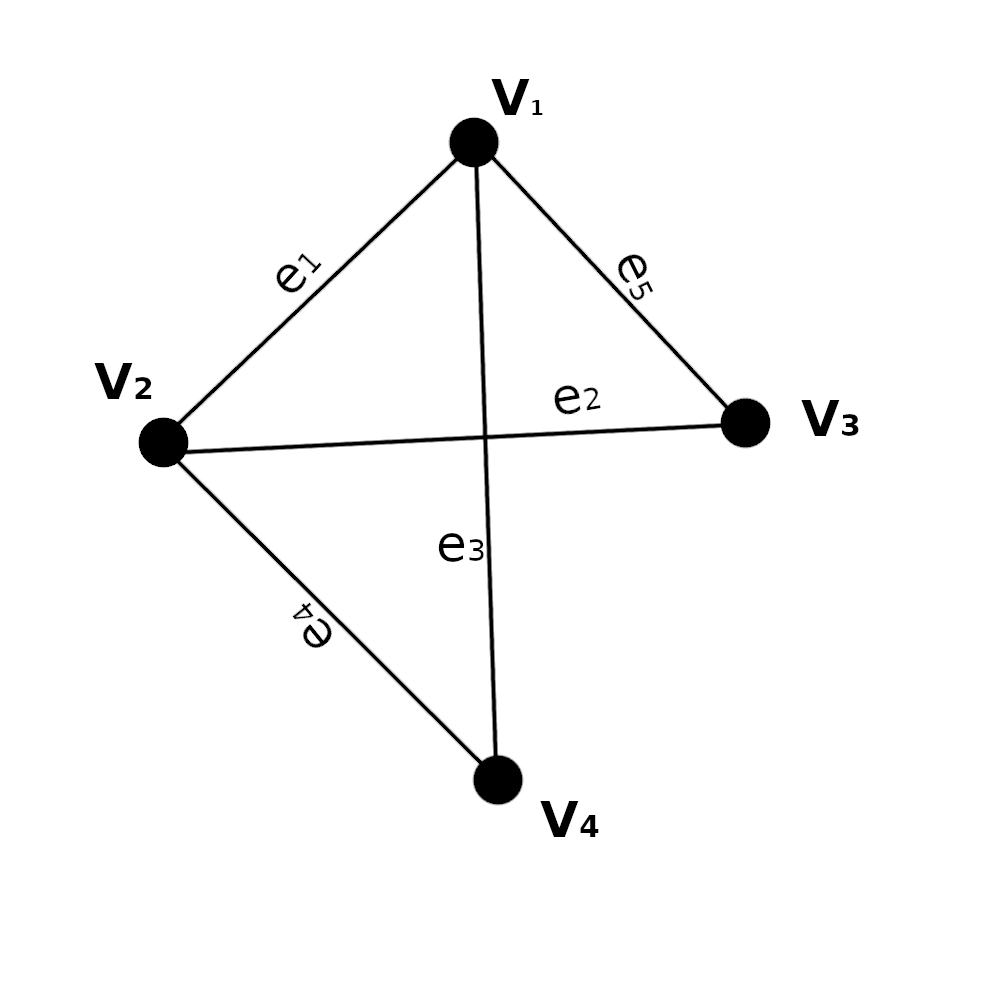
\includegraphics[scale=0.6]{grafo1}
	\\ Fonte: Compilação dos autores.
\end{figure}

Um \textit{caminho} é dado por uma sequência de vértices. Um \textit{ciclo} é um caminho através do qual é possível ``sair'' de um vértice e ``voltar'' para o mesmo por uma aresta diferente \cite[p. 519]{sedgewick}. Se este caminho for impossível, para todos os vértices, o grafo é dito \textit{acíclico}.

Um grafo é \textit{conexo} se existir pelo menos um caminho de qualquer vértice à qualquer outro vértice \cite[p. 519]{sedgewick}.

\subsection*{B. \quad Matriz de Incidência}

Uma forma conveniente de representar um grafo é pela chamada \textit{matriz de incidência}. Seja $G$ um grafo com $v$ vértices e $e$ arestas. $G$ pode ser escrito em termos de uma matriz $v \times e$, isto é, $M(G) = [m_{ij}]$, onde $m_{ij}$ (a entrada da matriz na i-ésima linha e na j-ésima coluna) representa quantas vezes (entre 0 e 2) $v_i$ e $e_j$ são \textit{incidentes}, ou seja, quantas vezes a aresta $e_j$ se ``encontra'' com o vértice $v_i$ \cite[p. 7]{bondy}. Dois vértices $v_a$ e $v_a$ possuem uma aresta $e_c$ entre si se e somente se $m_{ac} = m_{bc} \neq 0$.

A matriz de incidência que representa o grafo do exemplo anterior é, nesse caso:

\[
M(G) = 
\begin{bmatrix}
 & e_1 & e_2 & e_3 & e_4 & e_5 \\
 & - & - & - & - & - \\
 v_1 |& 1 & 0 & 1 & 0 & 1\\
 v_2 |& 1 & 1 & 0 & 1 & 0\\
 v_3 |& 0 & 1 & 0 & 0 & 1\\
 v_4 |& 0 & 0 & 1 & 1 & 0
\end{bmatrix}
\]

Verifica-se que, na matriz de incidência apresentada acima, $m_{11} = m_{21}$, o que indica que $e_1$ é uma conexão (aresta) entre $v_1$ e $v_2$. Nota-se também que três arestas incidem com $v_1$. 

\subsection*{C. \quad Árvore Geradora}

Por definição, uma \textit{árvore} é um grafo conexo acíclico \cite[p. 520]{sedgewick}, como explicitado na figura 2:

\begin{figure}[H]
	\caption{Exemplo de árvore} 
	\centering
	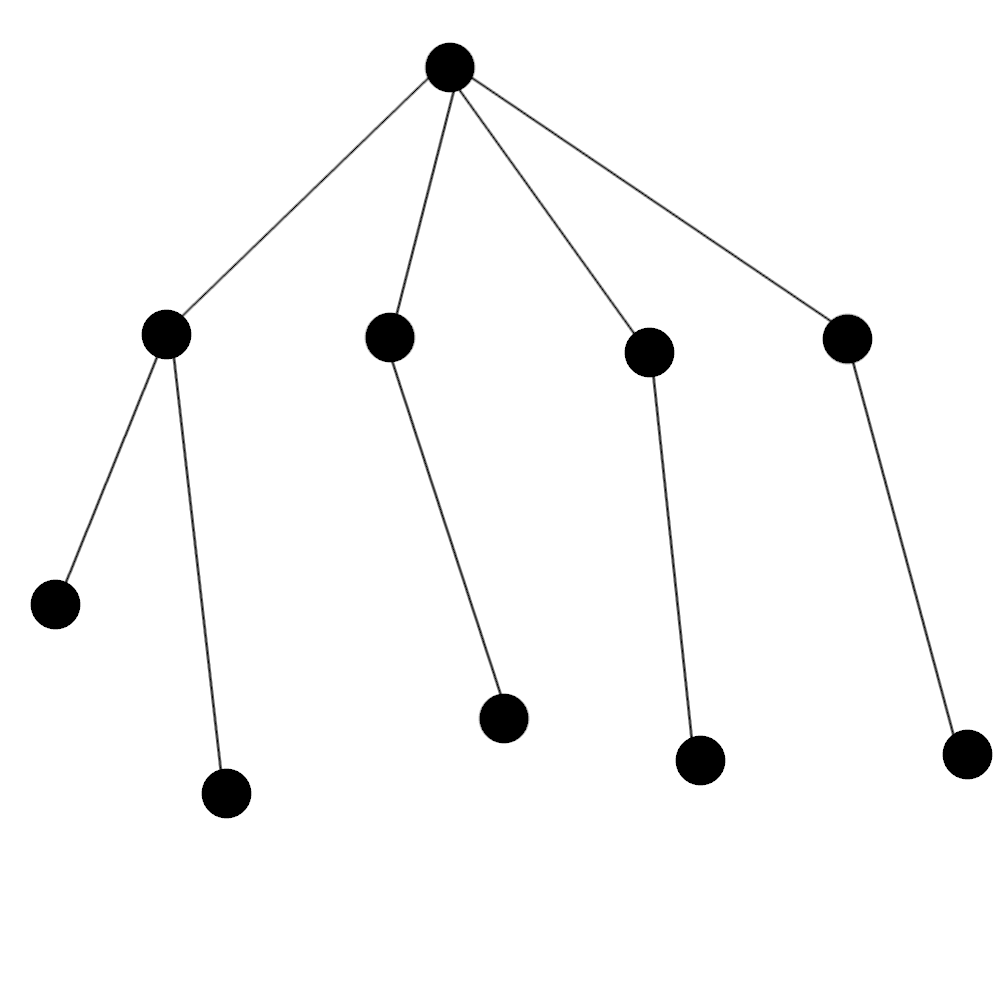
\includegraphics[scale=0.5]{tree1}
	\\ Fonte: Compilação dos autores.
\end{figure}

Uma \textit{árvore geradora} de um grafo conexo $G$ é um subgrafo que contém todos os vértices (e não necessariamente todas as arestas) de $G$ mas nenhum de seus ciclos. Uma árvore geradora do exemplo (1) pode ser:

\begin{figure}[H]
	\caption{Árvore geradora de (1)} 
	\centering
	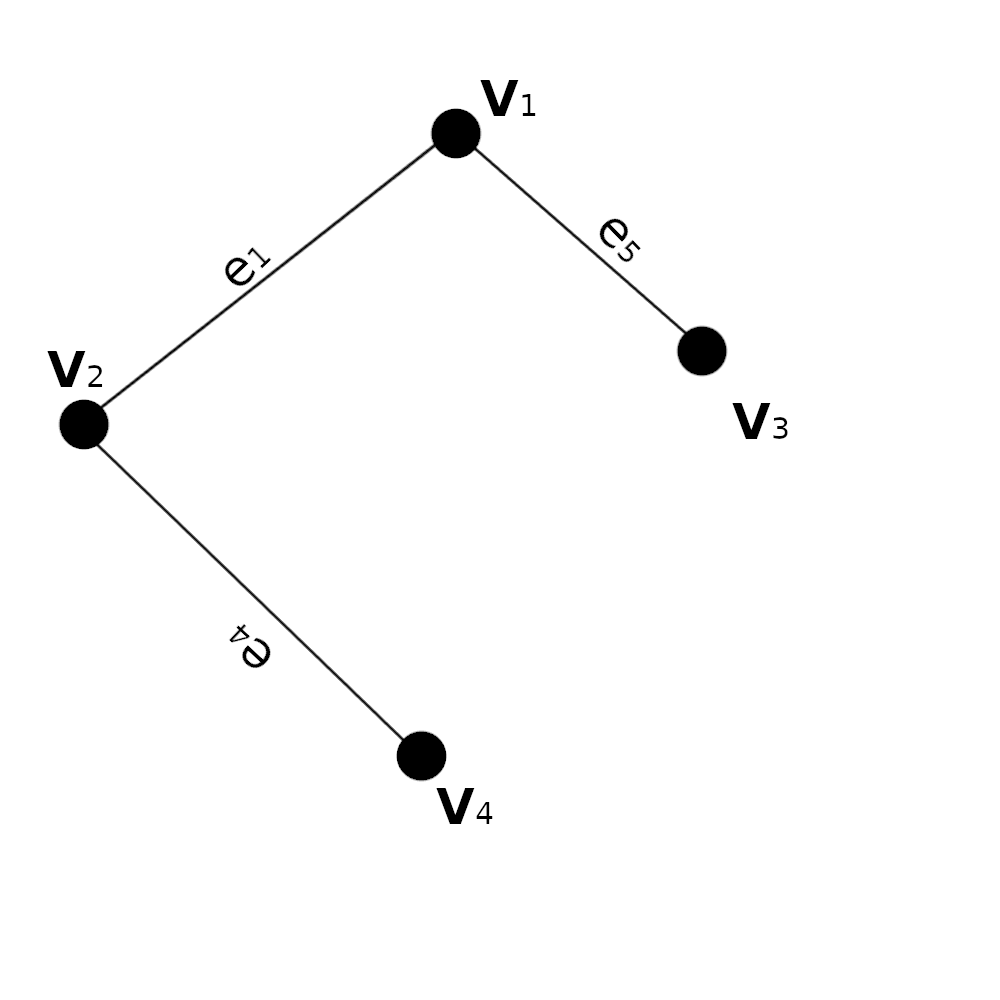
\includegraphics[scale=0.6]{spanning1}
	\\ Fonte: Compilação dos autores.
\end{figure}

Uma \textit{árvore co-geradora} de um grafo conexo $G$ é uma árvore formada pelas arestas (e seus respectivos vértices) que não aparecem na árvore geradora \cite[p. 834]{krishna}. Suas arestas são chamadas de \textit{acordes}. A árvore co-geradora do exemplo anterior é:

\begin{figure}[H]
	\caption{Árvore co-geradora de (1)} 
	\centering
	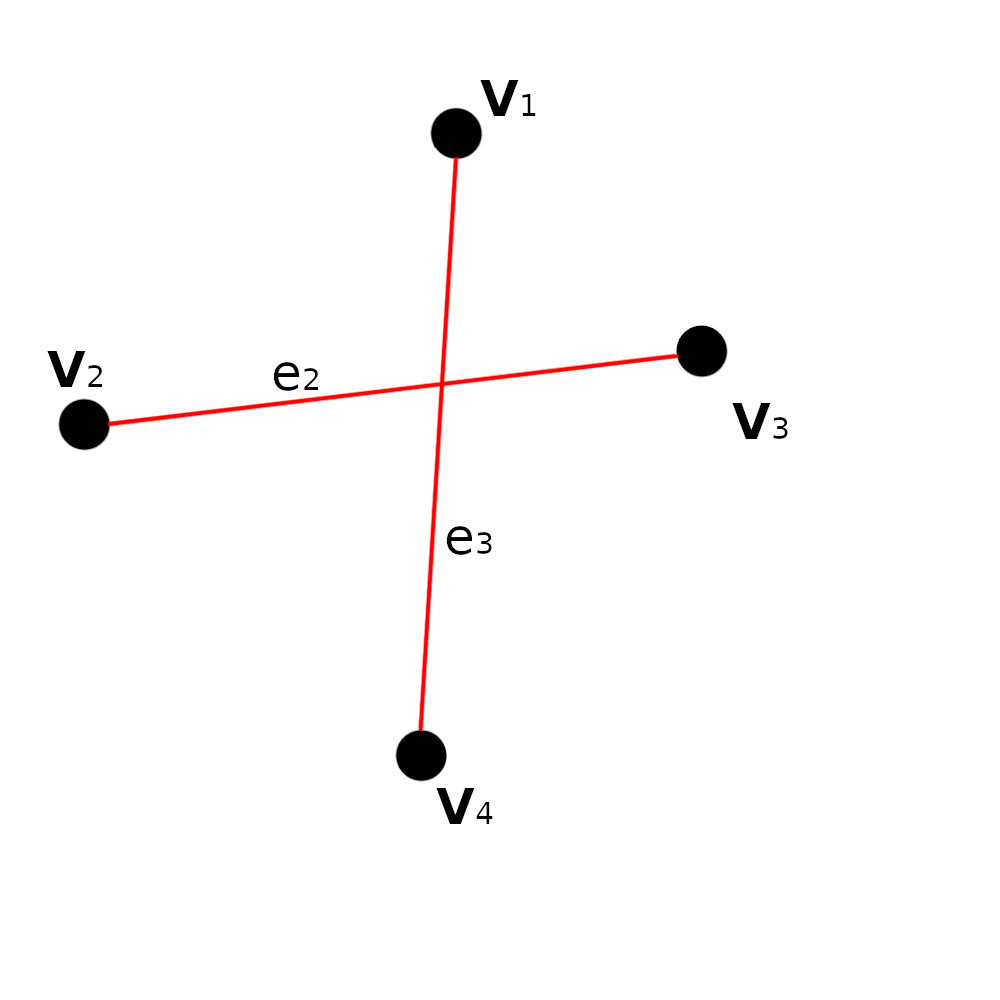
\includegraphics[scale=0.6]{cospanning1}
	\\ Fonte: Compilação dos autores.
\end{figure}

É possível ainda encontrar uma árvore geradora para qualquer grafo conexo computacionalmente. Para tal, basta realizar uma \textit{busca em profundidade} no grafo e então a árvore geradora será o caminho percorrido pela busca.

A busca em profundidade (ou DFS) consiste em dois passos simples: visitar um vértice inicial e recursivamente visitar todos os seus vizinhos ainda não visitados \cite[p. 531]{sedgewick}. Seja, por exemplo, o seguinte grafo $G$:

\begin{figure}[H]
	\caption{Exemplo (2) de um grafo} 
	\centering
	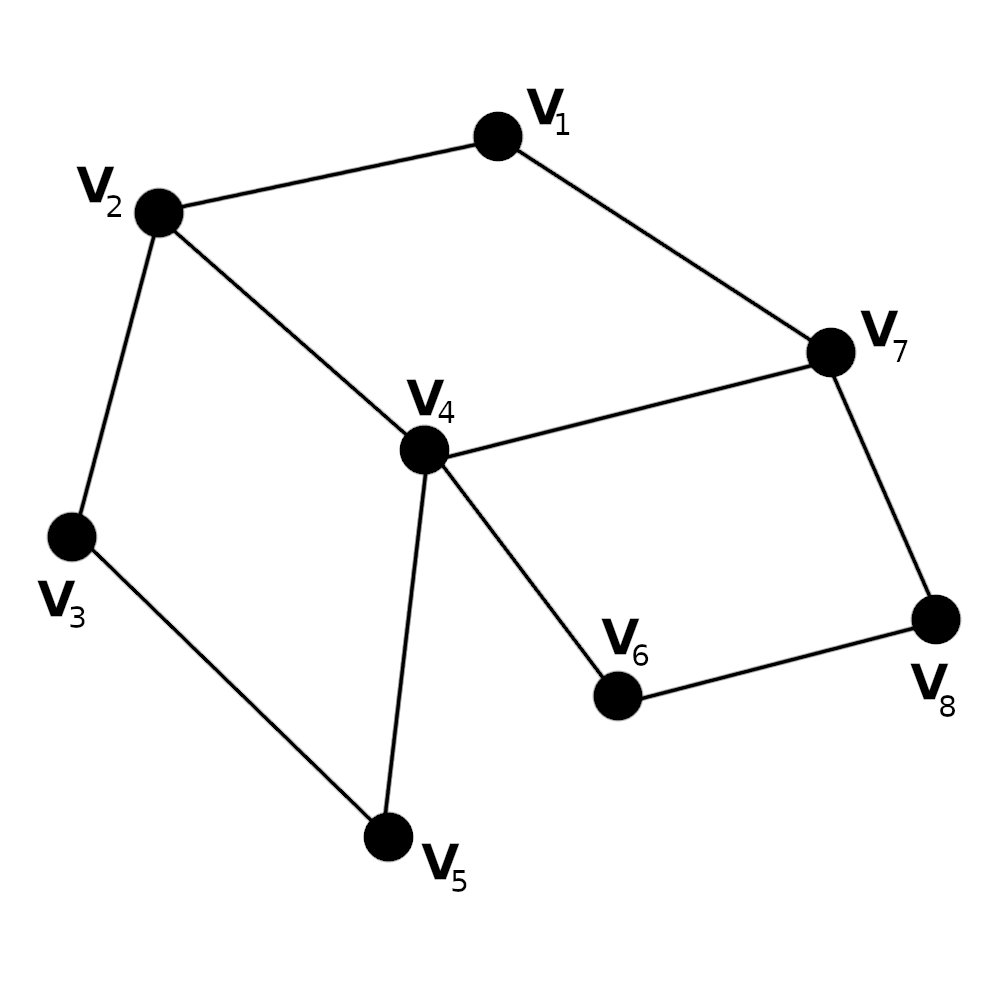
\includegraphics[scale=0.6]{grafo2}
	\\ Fonte: compilação dos autores.
\end{figure}

A seguinte figura mostra o percurso da DFS partindo de $v_1$, onde cada cor representa um passo do algoritmo:

\begin{figure}[H]
	\caption{DFS sobre (2)} 
	\centering
	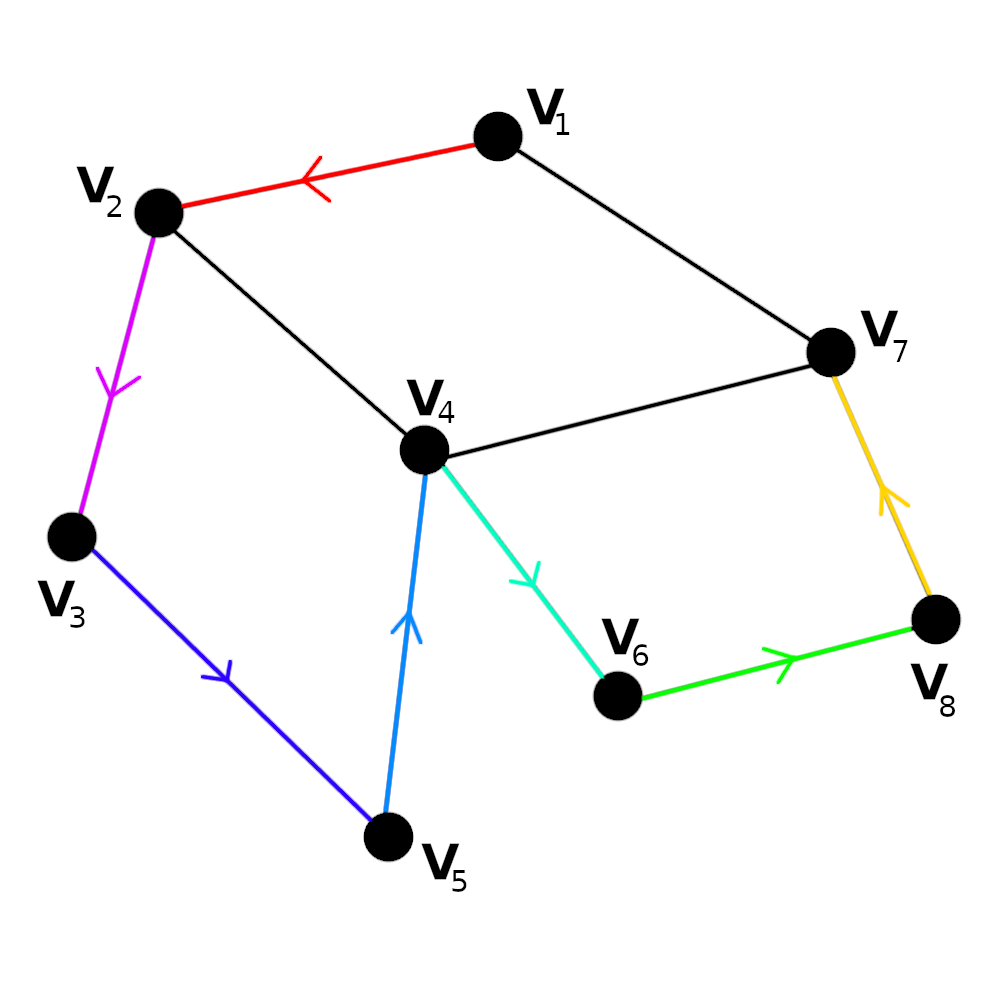
\includegraphics[scale=0.6]{dfs1}
	\\ Fonte: Compilação dos autores.
\end{figure}

É fácil perceber que o subgrafo formado pelas arestas destacadas é uma árvore geradora de $G$:

\begin{figure}[H]
	\caption{Arvore Gerada pela DFS} 
	\centering
	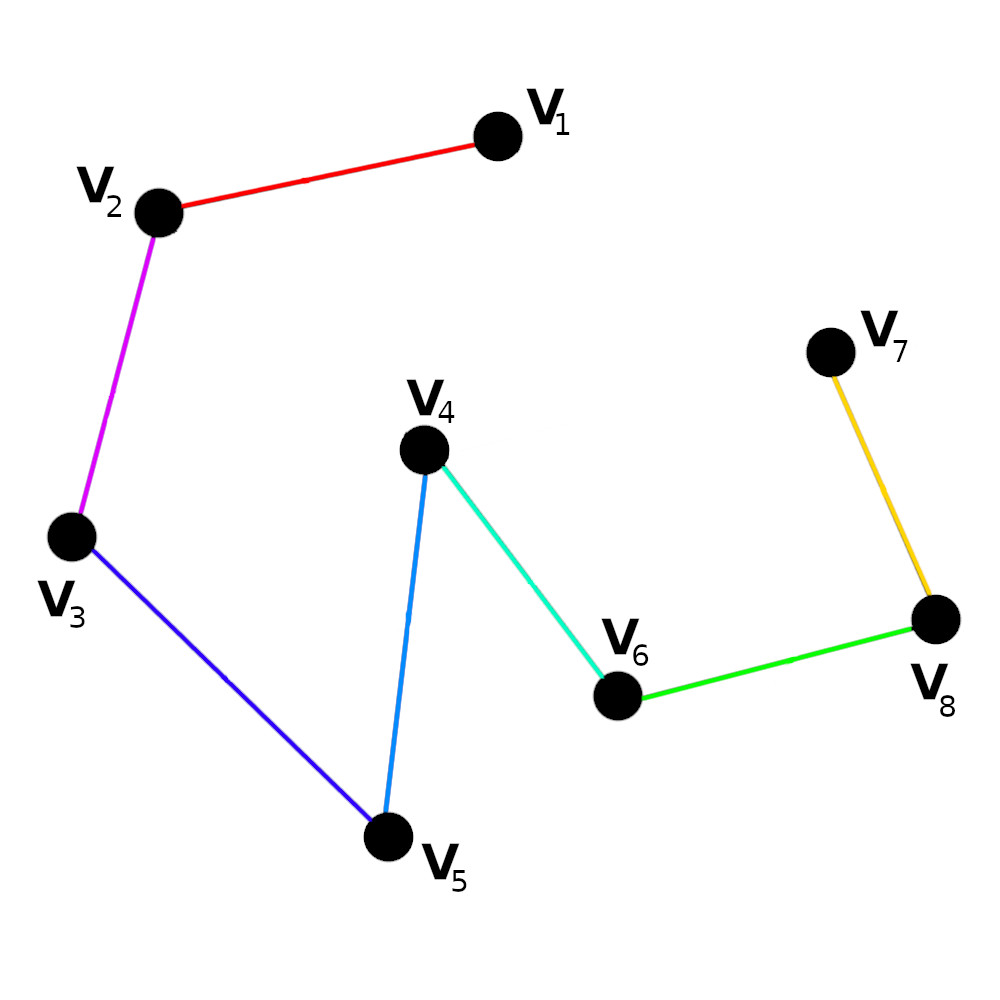
\includegraphics[scale=0.6]{spanning2}
	\\ Fonte: Compilação dos autores.
\end{figure}

O seguinte algoritmo representa uma implementação computacional do tópico discutido, assumindo um grafo conexo $G$ e uma árvore inicialmente vazia $T$:

\begingroup
\captionof{algorithm}{Árvore Geradora}\label{st}
\begin{algorithmic}[1]
\Function{arvoreGeradoraDFS}{$G$, $T$,$v$}
	\State{Marque $v$ como visitado}
	\State{Insira $v$ em $T$}
	\For{Todos os vizinhos $v_i$ não visitados de $v$}
		\State{Insira a aresta que conecta $v$ e $v_i$ em $T$}
		\State{arvoreGeradoraDFS($G$, $T$, $v_i$)}
	\EndFor
\EndFunction
\end{algorithmic}
\hrulefill
\endgroup

\subsection*{D. \quad Encontrando o Conjunto de Ciclos Fundamentais de um Grafo}

Assim como descrito por \cite{krishna}, ao adicionar um dos arcordes à árvore geradora de um grafo, obtém-se um grafo com exatamente um ciclo. Ao conjunto das arestas que formam este ciclo, dá-se o nome de ciclo fundamental. O conjunto dos ciclos obtidos ao se adicionar, separadamente, cada acorde à árvore geradora é denotado por conjunto fundamental de ciclos. 

A seguir, é apresentado um algoritmo para a obtenção do conjunto de ciclos fundamentais de um grafo, com base nas ideias apresentadas por \cite{krishna}. A ideia geral é encontrar uma árvore geradora $T$ do grafo $G$ e a cada passo inserir um \textit{acorde} $e_i \in (E(G)-E(T))$ em $T$, encontrar o ciclo gerado pela adição de $e_i$ (este processo pode ser facilmente implementado através de pequenas modificações no algoritmo de busca em profundidade), então, remover $e_i$ de $T$, até que todos os \textit{acordes} tenham passado pelo processo.

\begingroup
\captionof{algorithm}{Encontra Ciclos}\label{lp}
\begin{algorithmic}[1]
\Function{encontraCiclos}{$G$}
	\State{$T \gets arvoreGeradoraDFS(G, T, v_1)$}
	\For{Todas as arestas $e_i$ em $E(G)$}
		\State{Insira $e_i$ em $T$}
		\State{Encontre o único ciclo presente em $T$}
		\State{Remova $e_i$ de $T$}
	\EndFor
\EndFunction
\end{algorithmic}
\hrulefill
\endgroup

\subsection*{E. \quad Digrafo e Multigrafo}

Um grafo direcionado (ou digrafo) é um grafo no qual os vértices extremos de uma aresta podem (mas não necessariamente devem) estar conectados por uma via de mão única \cite[p. 566]{sedgewick}. Ou seja, dados dois vértices $v_1$ e $v_2$, uma aresta $e_1$ pode representar um caminho de $v_1$ à $v_2$ mas não necessariamente o contrário. Nesse caso, a aresta é chamada de \textit{arco}. Graficamente, os arcos são representados por setas que ligam dois vértices:

\begin{figure}[H]
	\caption{Exemplo de digrafo} 
	\centering
	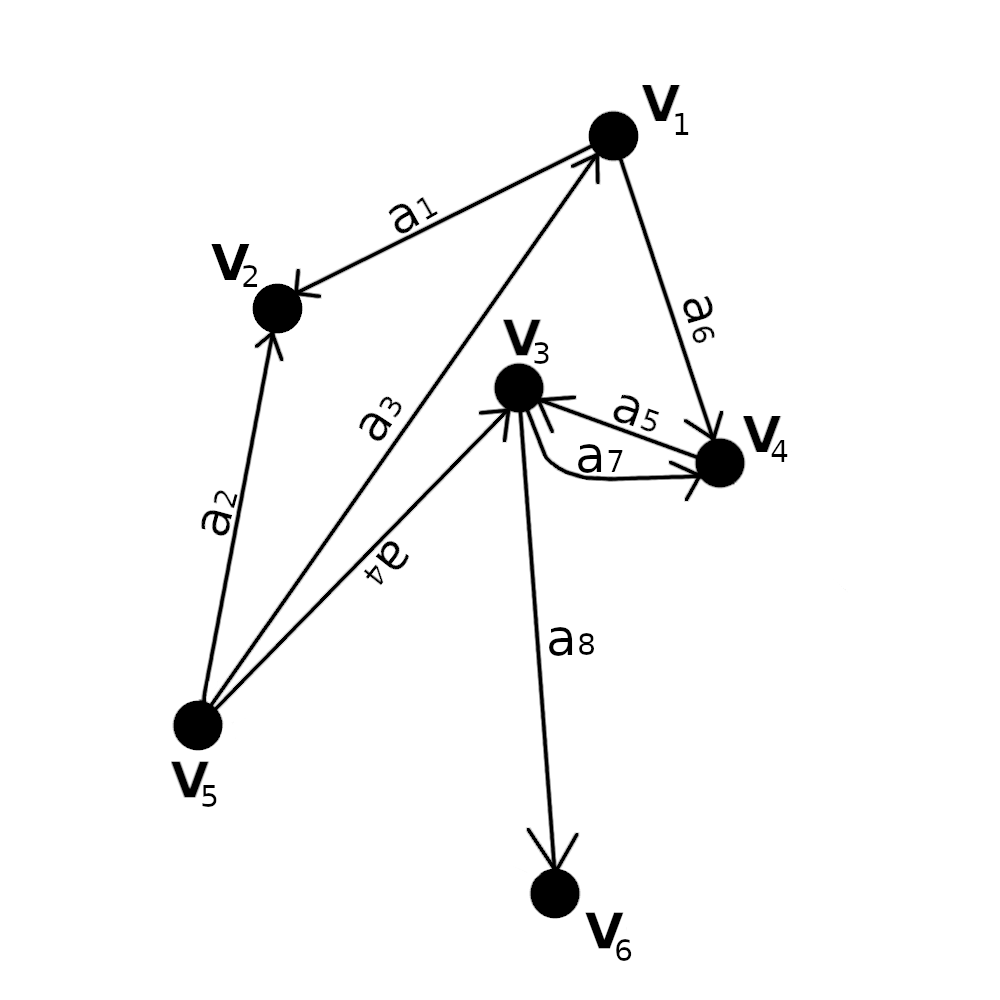
\includegraphics[scale=0.7]{digrafo1}
	\\ Fonte: Compilação dos autores.
\end{figure}

Convencionando $m_{ij} = 1$ se o arco $a_j$ \textit{sai} do vértice $v_i$ e $m_{ij} = -1$ se o arco $a_j$ \textit{chega} ao vértice $v_i$, a seguinte matriz de incidência representa o digrafo anterior:

\[\scriptsize
M = 
\begin{bmatrix}
 & a_1 & a_2 & a_3 & a_4 & a_5 & a_6 & a_7 & a_8 \\
 & - & - & - & - & - & - & - & - \\
 v_1 |& 1 & 0 & -1 & 0 & 0 & 1 & 0 & 0\\
 v_2 |& -1 & -1 & 0 & 0 & 0 & 0 & 0 & 0\\
 v_3 |& 0 & 0 & 0 & -1 & -1 & 0 & 1 & 1\\
 v_4 |& 0 & 0 & 0 & 0 & 1 & -1 & -1 & 0\\
 v_5 |& 0 & 1 & 1 & 1 & 0 & 0 & 0 & 0\\
 v_6 |& 0 & 0 & 0 & 0 & 0 & 0 & 0 & -1
\end{bmatrix}
\]

Note que há mais de um arco entre $v_3$ e $v_4$. A um grafo que permite esse tipo de comportamento se dá o nome de \textit{multigrafo}. 

\section{Circuitos Elétricos}

\subsection*{A. \quad Definição}

Segundo \cite[p. 4]{sadiku}, um \textit{circuito elétrico} é basicamente uma conexão entre componentes elétricos. Estes componentes são chamados de \textit{elementos} do circuito. Nesse trabalho são abordados apenas \textit{fontes de tensão constante} e \textit{resistores}.

Fontes de tensão constante são dispositivos que geram uma \textit{força eletromotriz} (ou diferença de potencial), ou seja, realizam \textit{trabalho} para deslocar \textit{cargas elétricas} \cite[p. 8]{sadiku}. A unidade da diferença de potencial (DDP) é o \textit{volt} ($V$) \cite[p. 9]{sadiku}. A esse deslocamento de cargas se dá o nome de \textit{corrente elétrica}, medida em \textit{ampères} (A) \cite[p. 6]{sadiku}.

Resistores são elementos que se submetidos à uma DDP, \textit{opõem-se} à passagem de corrente elétrica \cite[p. 28]{sadiku} de acordo com sua \textit{resistência}. Essas três quantidades são relacionadas pela \textit{Lei de Ohm}:

\[
V = R\cdot I
\]

Onde $V$ é a diferença de potencial, $R$ é a resistência do elemento resistivo e $I$ é a corrente que atravessa o elemento \cite[p. 28]{sadiku}.

\subsection*{B. \quad Diagramas}

É conveniente, ainda, representar os componentes elétricos graficamente para análise, sem ser necessário que se construa um circuito concreto.

A seguinte figura mostra como um resistor inserido entre dois pontos A e B pode ser representado:

\begin{figure}[H]
	\caption{Diagrama de um resistor} 
	\centering
	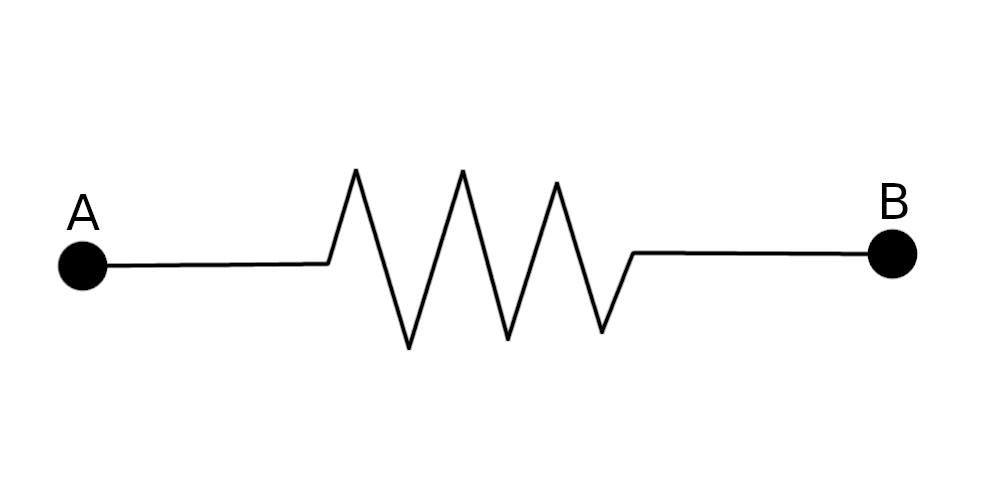
\includegraphics[scale=0.7]{res1}
	\\ Fonte: Compilação dos autores.
\end{figure}

A próxima figura expõe a representação gráfica de uma fonte de tensão constante entre A e B:

\begin{figure}[H]
	\caption{Diagrama de uma fonte de tensão} 
	\centering
	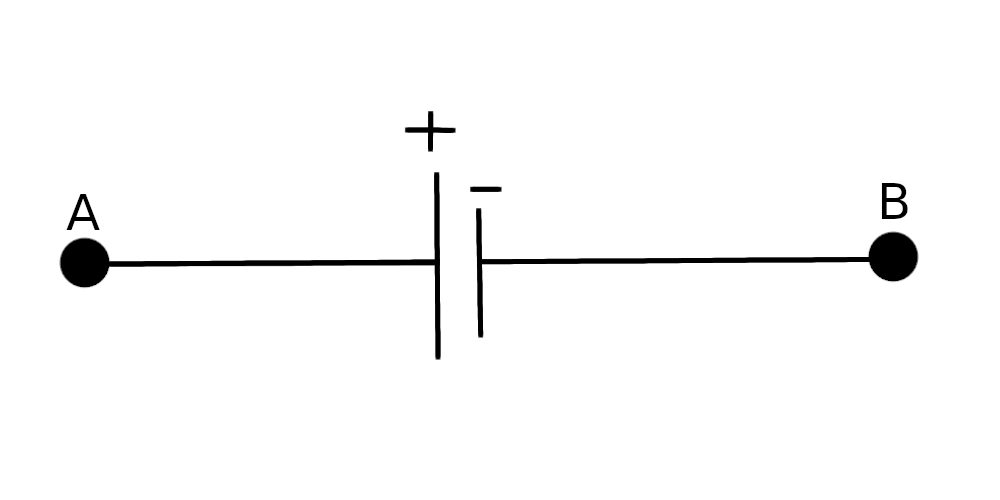
\includegraphics[scale=0.7]{vcc1}
	\\ Fonte: Compilação dos autores.
\end{figure}

Então, estes elementos podem ser combinados a fim de gerar circuitos mais complexos. A seguir, expõe-se um exemplo desse tipo:

\begin{figure}[H]
	\caption{Diagrama de um circuito resistivo} 
	\centering
	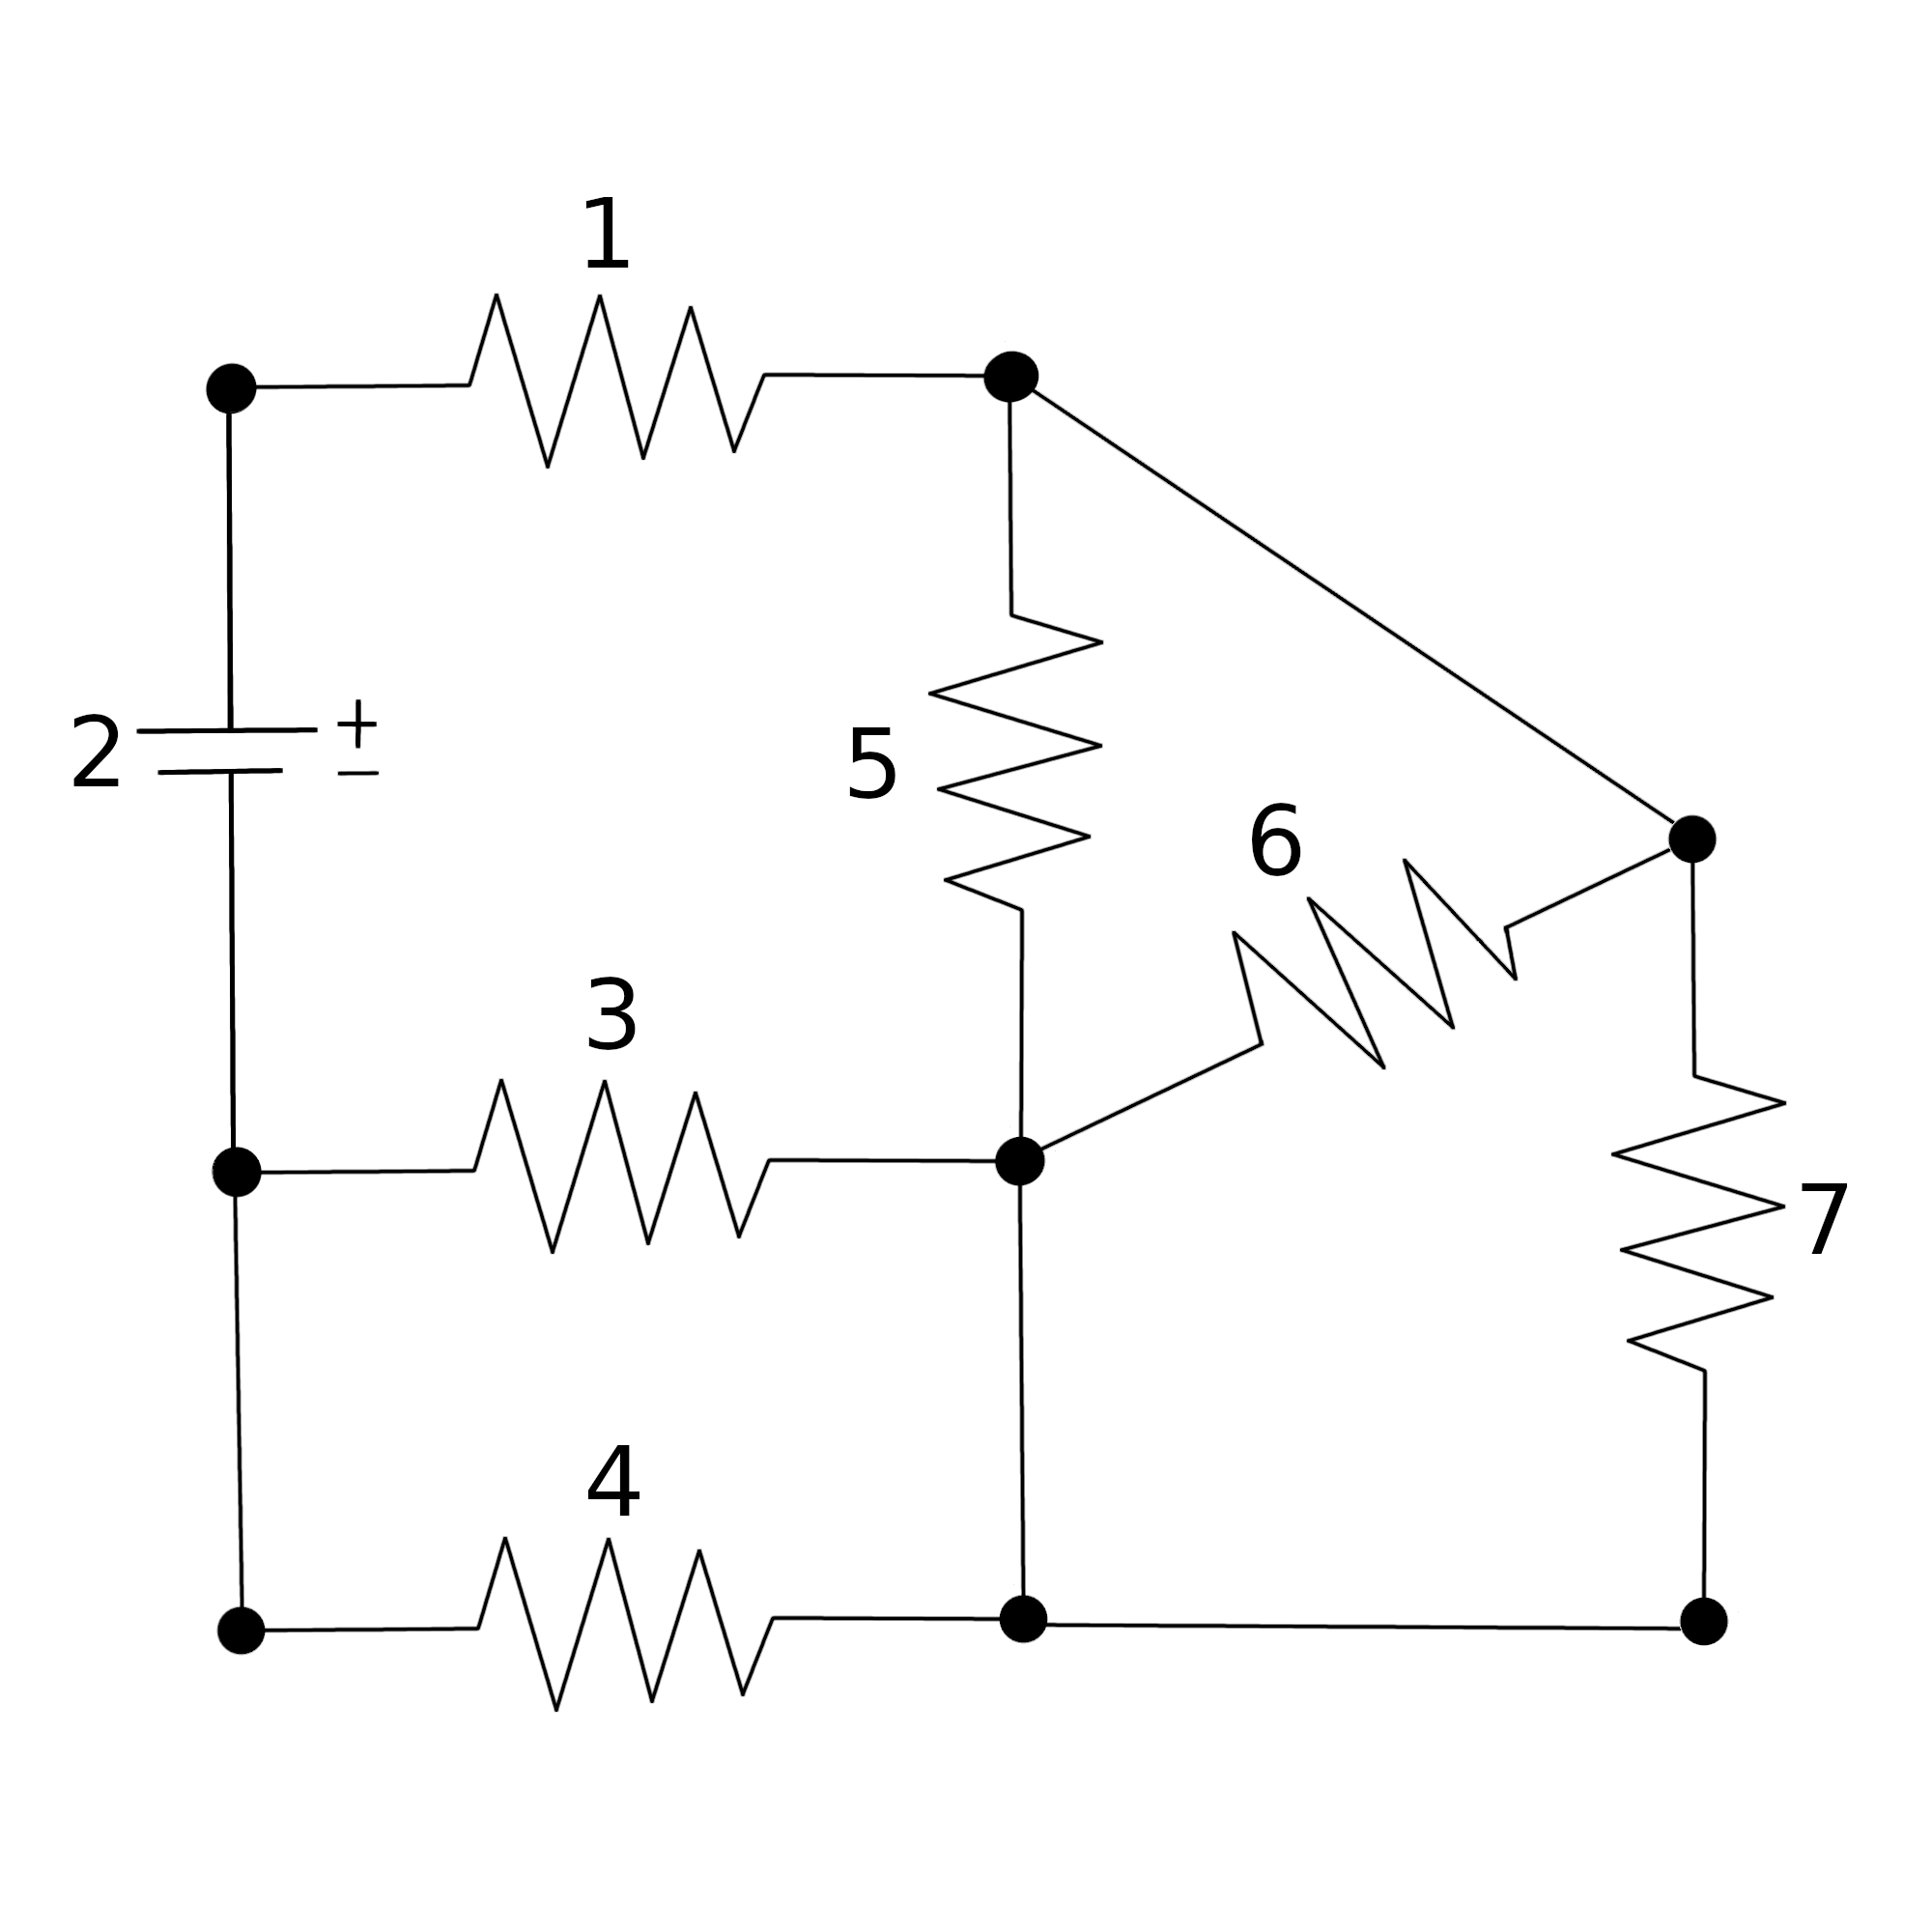
\includegraphics[scale=0.35]{circ1}
	\\ Fonte: Compilação dos autores.
\end{figure}


\subsection*{C. \quad Representação por Grafos}

Apesar dos diagramas serem convenientes para seres humanos visualizarem o comportamento de circuitos elétricos, a interpretação direta deles é muito difícil computacionalmente. Note, porém, que o diagrama é composto basicamente por vértices e arestas. Então, é possível redesenhar o diagrama como um digrafo, tomando os vértices como pontos sob diferentes potenciais e os arcos (com a mesma numeração) como os componentes elétricos, assim como mostrado por \cite[p. 838]{krishna}. Então, o seguinte grafo representa o circuito anterior:

\begin{figure}[H]
	\caption{Grafo do circuito resistivo} 
	\centering
	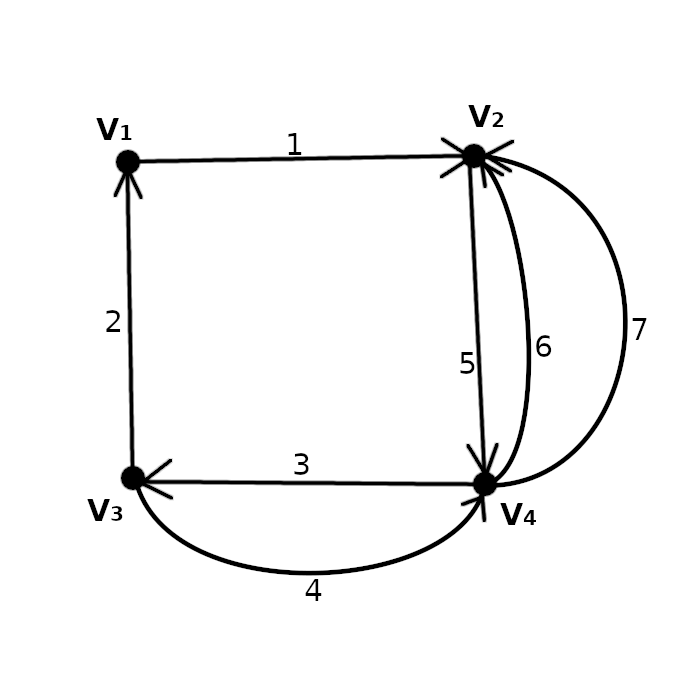
\includegraphics[scale=1]{grcrc1}
	\\ Fonte: Compilação dos autores.
\end{figure}

O sentido dos arcos representa o sentido da corrente que será assumido na simulação. Então, a matriz de incidência resultante é:

\[
M = 
\begin{bmatrix}
 & a_1 & a_2 & a_3 & a_4 & a_5 & a_6 & a_7 \\
 & - & - & - & - & - & - & - \\
 v_1 |& 1  & -1 & 0  & 0  & 0  & 0  & 0  \\
 v_2 |& -1 & 0  & 0  & 0  & 1  & -1 & -1 \\
 v_3 |& 0  & 1  & -1 & 1  & 0  & 0  & 0  \\
 v_4 |& 0  & 0  & 1  & -1 & -1 & 1  & 1  \\
\end{bmatrix}
\]

Os arcos que se incidem nos mesmos dois vértices são componentes em \textit{paralelo}. Dois arcos que formam um caminho $v_i - v_j$, $v_j - v_k$, sendo os únicos arcos incidentes entre $v_i$, $v_j$ e $v_j$, $v_k$, são dois componentes em \textit{série}.

\subsection*{D. \quad Solução Computacional}

\textit{Resolver} um circuito elétrico consiste em utilizar o \textit{princípio de conservação da carga elétrica} e o \textit{princípio de conservação de energia} para encontrar todas as variáveis desconhecidas dos componentes. Comumente são conhecidas apenas a tensão da fonte e as resistências dos resistores.

O método utilizado neste artigo consiste em uma adaptação dos métodos expostos em \cite{krishna} e \cite{boruah}.

A \textit{Lei das Tensões de Kirchhoff} é a aplicação do princípio de conservação de energia aos circuitos elétricos e diz que \cite[p. 945]{boruah}:

\[
\sum_{k=1}^{e} b_{rk}V_k = 0
\]

Onde $e$ é o número de arcos do grafo, $b_{rk}$ é a entrada na posição $rk$ da matriz $B$ dos ciclos de $G$ e $V_k$ é a tensão através de um arco. Em outras palavras, diz que a soma das tensões em um ciclo é nula.

Já a \textit{Lei das Correntes de Kirchhoff} enuncia o emprego do princípio da conservação de carga elétrica aos circuitos elétricos da seguinte forma \cite[p. 945]{boruah}:

\[
\sum_{k=1}^{e} a_{rk}I_k = 0
\]

Onde $a_{rk}$ é a entrada na posição $rk$ da matriz de incidência $A$ do grafo $G$, $I_k$ é a corrente que flui pela aresta $k$ e $e$ é o número de arcos do grafo. Em outras palavras, diz que a soma das correntes em um nodo é nula.

A matriz $B$ dos ciclos fundamentais é uma matriz onde cada linha representa um ciclo fundamental do grafo $G$ e cada coluna representa um arco presente no ciclo de acordo com as seguintes regras \cite[p. 948]{boruah}:

\begin{itemize}
	\item $b_{ij} = 1$ se o galho $b_j$ pertence ao ciclo fundamental $c_i$ e sua referência têm a mesma orientação;
	\item $b_{ij} = -1$ se o galho $b_j$ pertence ao  ciclo fundamental $c_i$ e sua referência têm orientações opostas;
	\item $b_{ij} = 0$ se o galho $b_j$ não pertence ao ciclo fundamental $c_i$.
\end{itemize}

A matriz $R$ das resistências é uma matriz diagonal quadrada $e \times e$, onde $e$ é o número de arcos no grafo, cujos elementos $r_{ii}$ representam a resistência no arco $i$.

Seja $V$ a matriz coluna que representa as tensões das fontes de corrente contínua do circuito, $R$ a matriz das resistências e $I_b$ a matriz coluna que representa as correntes em cada um dos galhos (arestas) do circuito, tem-se, pela lei das tensões de kirchoff:

\[
B(V -RI_b) = 0
\]

\[
\iff 
 BV = BRI_b  
\]

Mas, sabemos que $I_b = B^tI_L$, onde $I_L$ é a matriz de correntes em cada ciclo fundamental e $B^t$ é a transposta de $B$. Então:

\[
BV = BRB^tI_L
\]

Como $B$, $R$ e $B^t$ são conhecidos e formam uma matriz quadrada, $I_L$ é uma matriz coluna de incógnitas e $BV$ é uma matriz coluna de constantes, a equação anterior é equivalente a um sistema linear na forma $Ax = b$. Logo, basta resolver o sistema e substituir em $I_b = B^tI_L$ para encontrar todas as correntes.

Desta forma, neste artigo, utilizou-se o seguinte algoritmo para a solução computacional de circuitos elétricos, assumindo $A$ como a matriz de incidência do grafo, $R$ como a matriz de resistência, $B$ como a matriz dos ciclos fundamentais, $I$ como a matriz das correntes e $V$ como a matriz das tensões das fontes:

\begingroup
\captionof{algorithm}{Solucionador de Circuitos}\label{cs}
\begin{algorithmic}[1]
\Function{resolveCircuito}{$A$, $R$, $B$, $I$, $V$}
	\State{$B \gets encontraCiclos(A)$}
	\State{$M \gets BR_bB^t$}
	\State{$n \gets BV_s$}
	\State{$x^{(0)}\gets$ vetor nulo}
	\If{$M$ atende ao critério de Sassenfeld}
		\State{$I_L \gets gaussSeidel(M, n, x^{(0)}, 10^{-8}, 10^3)$}
	\Else
		\State{$I_L \gets gaussJordan(M, n)$}
	\EndIf
	\State{$I_b \gets B^tI_L$}
\EndFunction
\end{algorithmic}
\hrulefill
\endgroup

Ao fim do algoritmo, são conhecidas todas as correntes e tensões e, portanto, o circuito passa a ser determinado.


\section{RESULTADOS}

Considere o seguinte circuito, onde a tensão na fonte é de $5V$ e todos os resistores possuem resistência de $100 \Omega$:

\begin{figure}[H]
	\caption{Exemplo (1) de circuito} 
	\centering
	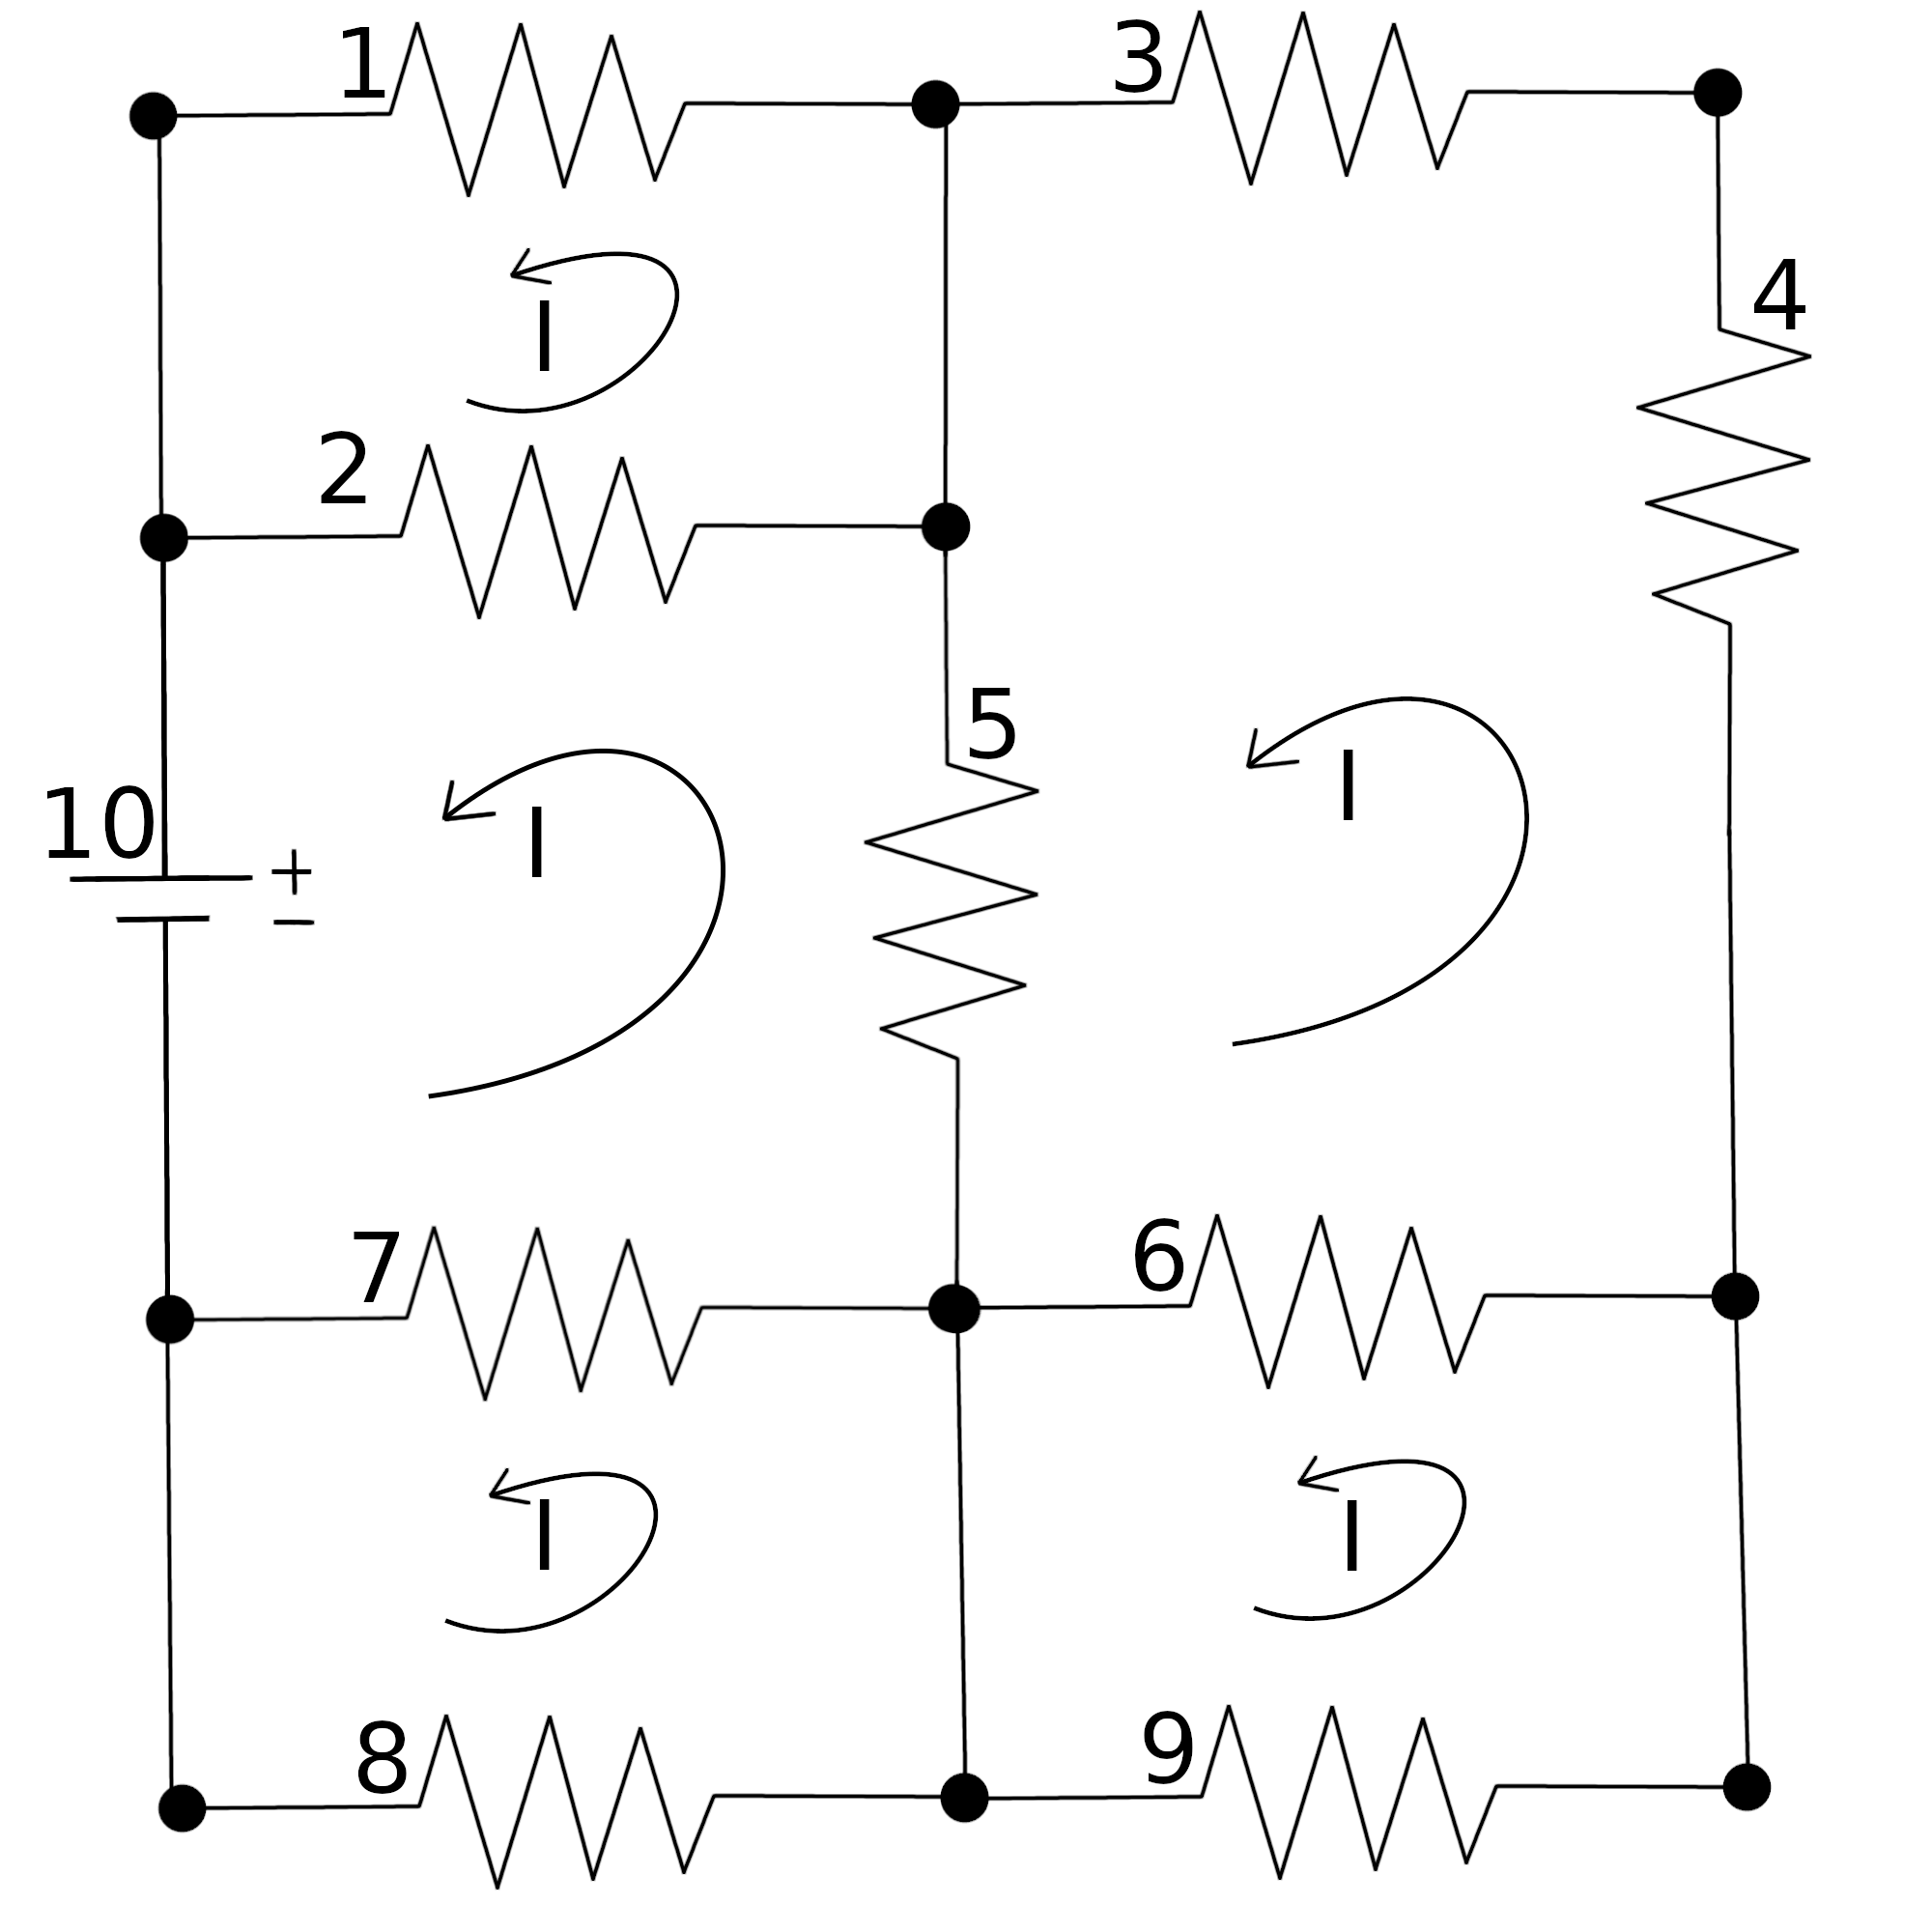
\includegraphics[scale=0.35]{circ2}
	\\ Fonte: Compilação dos autores.
\end{figure}

É possível aplicar a lei das Tensões de Kirchhoff para cada malha, que resulta no seguinte sistema:

\[
\left\{
\begin{aligned}
    V_1 + V_2 &= \,0 \\ 
  	V_{10} + V_7 + V_5 + V_2 &= \,0 \\ 
	V_3 + V_4 + V_5 + V_6 &= \,0 \\
	V_7 + V_8 &= \,0 \\ 
	V_6 + V_9 &= \,0 
\end{aligned}
\right.
\]

As correntes do circuito podem ser desenhadas, assumindo um sentido arbitrário e o sentido anti-horário como positivo, da seguinte forma:

\begin{figure}[H]
	\caption{Correntes de (1)} 
	\centering
	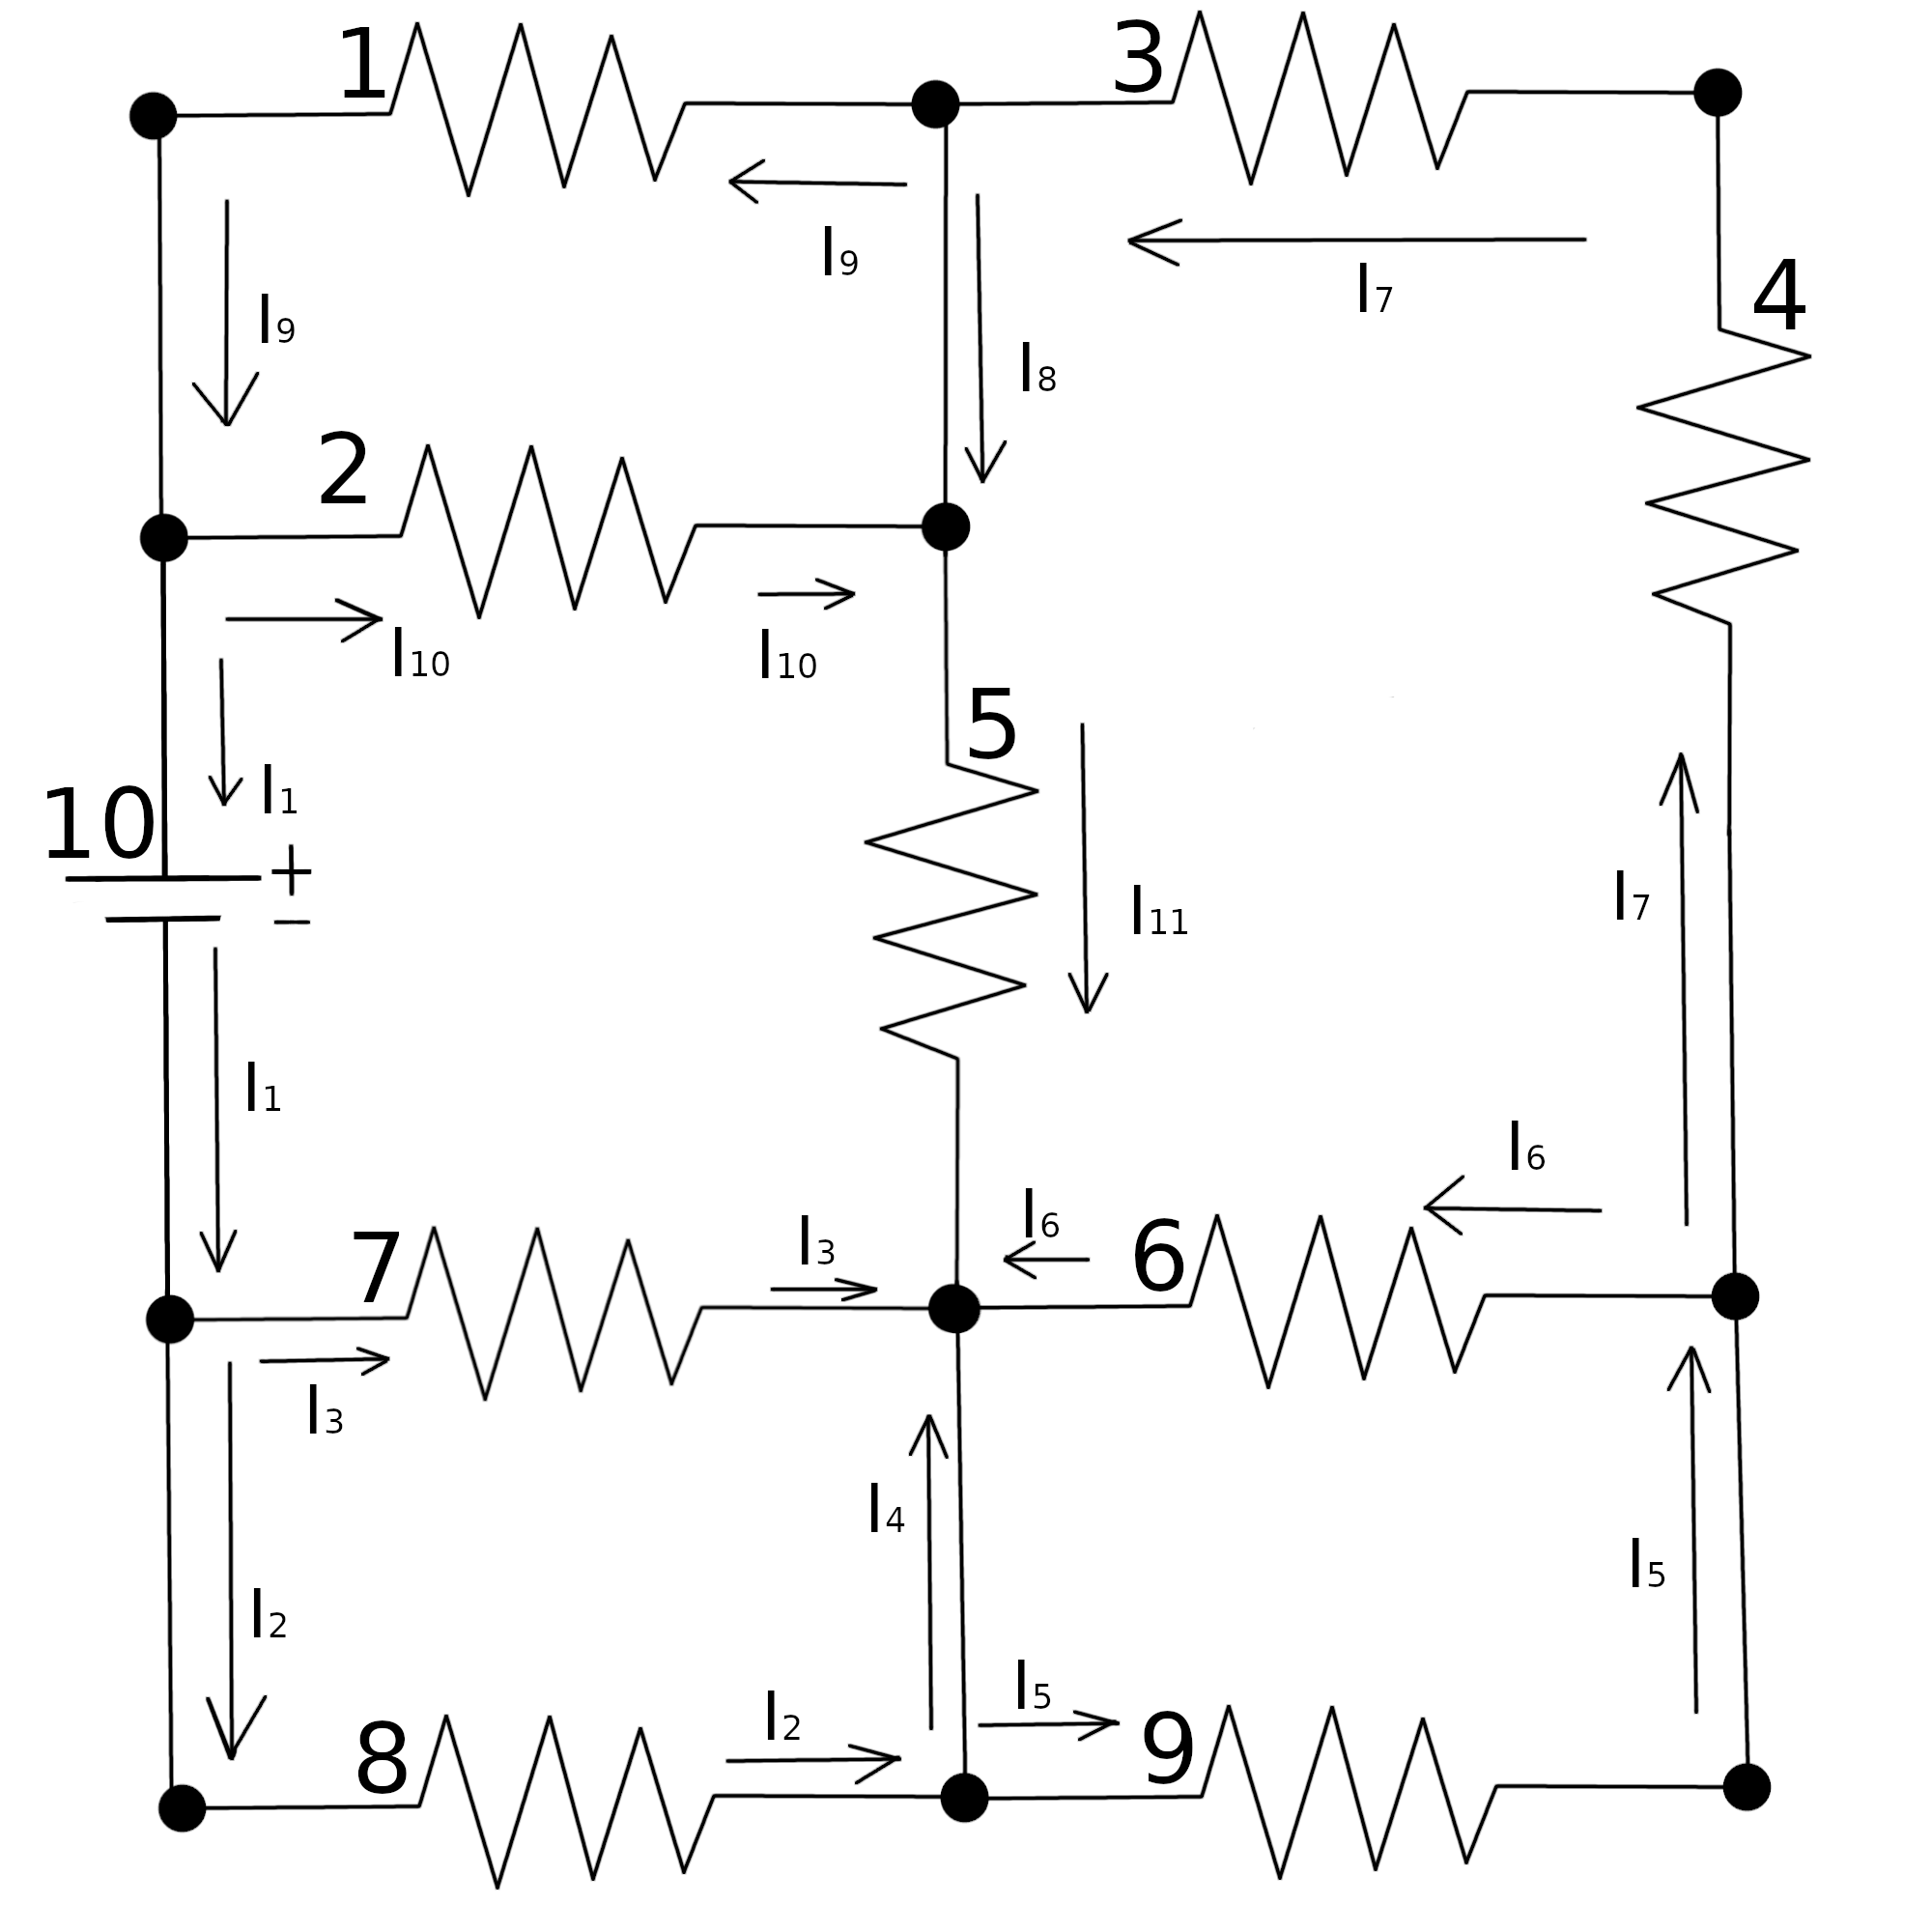
\includegraphics[scale=0.43]{circ22}
	\\ Fonte: Compilação dos autores.
\end{figure}

Então, pode-se aplicar a lei das correntes de Kirchhoff ao circuito. Tem-se, então, o seguinte sistema:

\[
\left\{
\begin{aligned}
    I_1 - I_2 - I_3 &= \, 0 \\
    I_2 - I_4 - I_5 &= \, 0 \\
    I_5 - I_6 - I_7 &= \, 0 \\
    I_3 + I_4 + I_6 + I_{11} &= \, 0 \\
    I_7 - I_8 - I_9 &= \, 0 \\
    - I_1 + I_9 - I_{10} + &= \, 0 \\
    I_8 + I_{10} - I_{11} &= \, 0 
\end{aligned}
\right.
\]

É possível ainda reescrever o primeiro sistema em função da Lei de Ohm:

\[
\left\{
\begin{aligned}
    I_9R + I_{10}R &= \,0 \\ 
    V_{10} - I_3R + I_{10}R + I_{11}R &= \,0 \\ 
	-I_7R - I_7R + I_6R - I_{11}R &= \,0 \\
	- I_3R + I_2R &= \,0 \\ 
	I_5R + I_6R &= \,0
\end{aligned}
\right.
\]

Que pode ser juntado com o segundo sistema:

\[
\left\{
\begin{aligned}
    I_9R + I_{10}R &= \,0 \\ 
    V_{10} - I_3R + I_{10}R + I_{11}R &= \,0 \\ 
	-I_7R - I_7R + I_6R - I_{11}R &= \,0 \\
	- I_3R + I_2R &= \,0 \\ 
	I_5R + I_6R &= \,0 \\
	I_1 - I_2 - I_3 &= \, 0 \\
    I_2 - I_4 - I_5 &= \, 0 \\
    I_5 - I_6 - I_7 &= \, 0 \\
    I_3 + I_4 + I_6 + I_{11} &= \, 0 \\
    I_7 - I_8 - I_9 &= \, 0 \\
    - I_1 + I_9 - I_{10} + &= \, 0 \\
    I_8 + I_{10} - I_{11} &= \, 0 
\end{aligned}
\right.
\]

Substituindo $V_{10}$ e $R$ e resolvendo para o vetor I, notando que os sinais negativos indicam uma escolha equivocada de sentido inicial para a corrente, temos:

\[
I = 
\begin{bmatrix}
0,0291 \bar 6 & \\
0,01458 \bar 3  & \\
0,01458 \bar 3  & \\
0,010417  & \\
0,0041 \bar 6  & \\
-0,0041 \bar 6  & \\
0,008 \bar 3  & \\
-0,00625  & \\
0,01458\bar 3  & \\
-0,01458\bar 3  & \\
-0,0208\bar 3  & \\
\end{bmatrix}
\]

Este mesmo circuito pode ser resolvido computacionalmente de forma trivial. Basta inserí-lo no programa desenvolvido para este artigo e checar os resultados, da seguinte forma:

\begin{figure}[H]
	\caption{Simulação de (1)} 
	\centering
	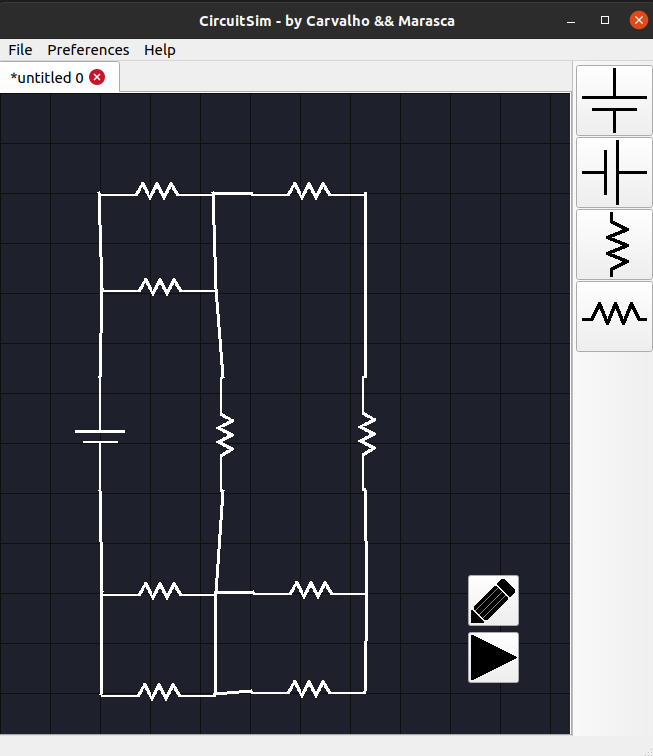
\includegraphics[scale=0.2]{circuitsim1}
	\\ Fonte: Compilação dos autores.
\end{figure}

Com o mesmo sentido de corrente assumido, são dadas as seguintes correntes nos componentes:

\begin{figure}[H]
	\caption{Corrente na fonte} 
	\centering
	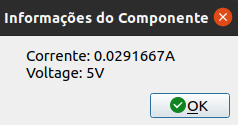
\includegraphics[scale=0.7]{iv}
	\\ Fonte: Compilação dos autores.
\end{figure}

\begin{figure}[H]
	\caption{Corrente em $R_1$} 
	\centering
	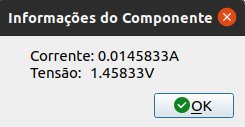
\includegraphics[scale=0.7]{ir1}
	\\ Fonte: Compilação dos autores.
\end{figure}

\begin{figure}[H]
	\caption{Corrente em $R_2$} 
	\centering
	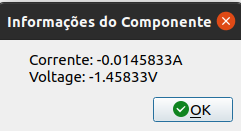
\includegraphics[scale=0.7]{ir2}
	\\ Fonte: Compilação dos autores.
\end{figure}

\begin{figure}[H]
	\caption{Corrente em $R_3$} 
	\centering
	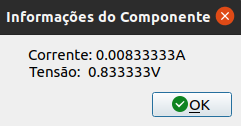
\includegraphics[scale=0.7]{ir3}
	\\ Fonte: Compilação dos autores.
\end{figure}

\begin{figure}[H]
	\caption{Corrente em $R_4$} 
	\centering
	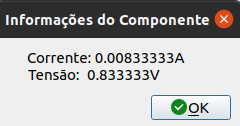
\includegraphics[scale=0.7]{ir4}
	\\ Fonte: Compilação dos autores.
\end{figure}

\begin{figure}[H]
	\caption{Corrente em $R_5$} 
	\centering
	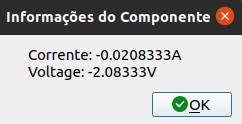
\includegraphics[scale=0.7]{ir5}
	\\ Fonte: Compilação dos autores.
\end{figure}

\begin{figure}[H]
	\caption{Corrente em $R_6$} 
	\centering
	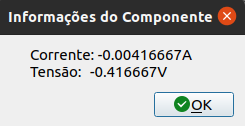
\includegraphics[scale=0.7]{ir6}
	\\ Fonte: Compilação dos autores.
\end{figure}

\begin{figure}[H]
	\caption{Corrente em $R_7$} 
	\centering
	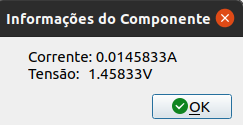
\includegraphics[scale=0.7]{ir7}
	\\ Fonte: Compilação dos autores.
\end{figure}

\begin{figure}[H]
	\caption{Corrente em $R_8$} 
	\centering
	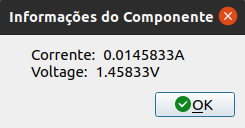
\includegraphics[scale=0.7]{ir8}
	\\ Fonte: Compilação dos autores.
\end{figure}

\begin{figure}[H]
	\caption{Corrente em $R_9$} 
	\centering
	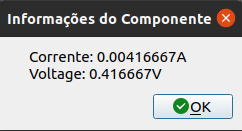
\includegraphics[scale=0.7]{ir9}
	\\ Fonte: Compilação dos autores.
\end{figure}

Note que apesar de não haver diferenças entre os resultados obtidos pela simulação e os resultados obtidos manualmente, a simulação pode gerar erros de arredondamento devido à representação numérica de ponto flutuante utilizada pelos computadores. Conforme \cite{chapra}, a fonte destes erros decorre, principalmente, da limitação de quantidades que podem representadas pelo sistema de ponto flutuante.
\section{CONCLUSÃO}

Então, conclui-se que, embora seja necessário o estudo de diversos tópicos para realizar a implementação, o resultado final é satisfatório, já que apresenta a solução exata do problema proposto, facilitando e acelerando a obtenção destes resultados. 

Vale ressaltar ainda que seria possível expandir os assuntos aqui discutidos a fim de produzir um solucionador que abranja mais tipos de componentes. Contudo, o objetivo inicial de simular circuitos resistivos alimentados por fontes de corrente contínua, o que foi alcançado de forma suficientemente satisfatória.

\newpage

\renewcommand{\refname}{REFERÊNCIAS}
\bibliography{bibliografia}

\end{document}